\documentclass[12pt,a4paper]{report}
\usepackage{enumerate}
\usepackage{amsmath}
\usepackage{mathrsfs}
\usepackage{amsmath}
\usepackage{graphicx} 



\title{Social Analysis Study on DeviantArt}

\date{\emph{10.06.2011} \\ \emph{Version 5.0} }

\author{CmpE 492 Project\\
	By: Ferhat Elmas \\
	Student Id: 2006101102\\
	Advisor: Haluk Bing\"{o}l
}

\begin{document}
\pagenumbering{roman}


\maketitle

\begin{table}[htdp]
\begin{center}
\textup{\Huge Version History}
\begin{tabular}{|c|c|p{10cm}|}
\hline
\textbf{Version} & \textbf{Date} & \textbf{Explanation} \\
\hline
1.0 & 30.03.2011 & Algorithm Design and Specification \\
\hline
2.0& 22.04.2011 & Some errors (keyword, logic, notation) are fixed, the details of the distributions of the user and resource generation and a table of some basic properties of distributions are added, algorithm is improved and details are added\\
\hline
3.0& 27.04.2011& Parameter Analysis is added\\
\hline
4.0& 04.05.2011& Notation is improved, appendix is added, design of the chapters is changed\\
\hline
5.0& 10.06.2011& Analysis of Real Data Chapter is added and simulation results are compared to real findings\\
\hline
\end{tabular}
\end{center}
\end{table}

\clearpage

\hspace{-3.7cm}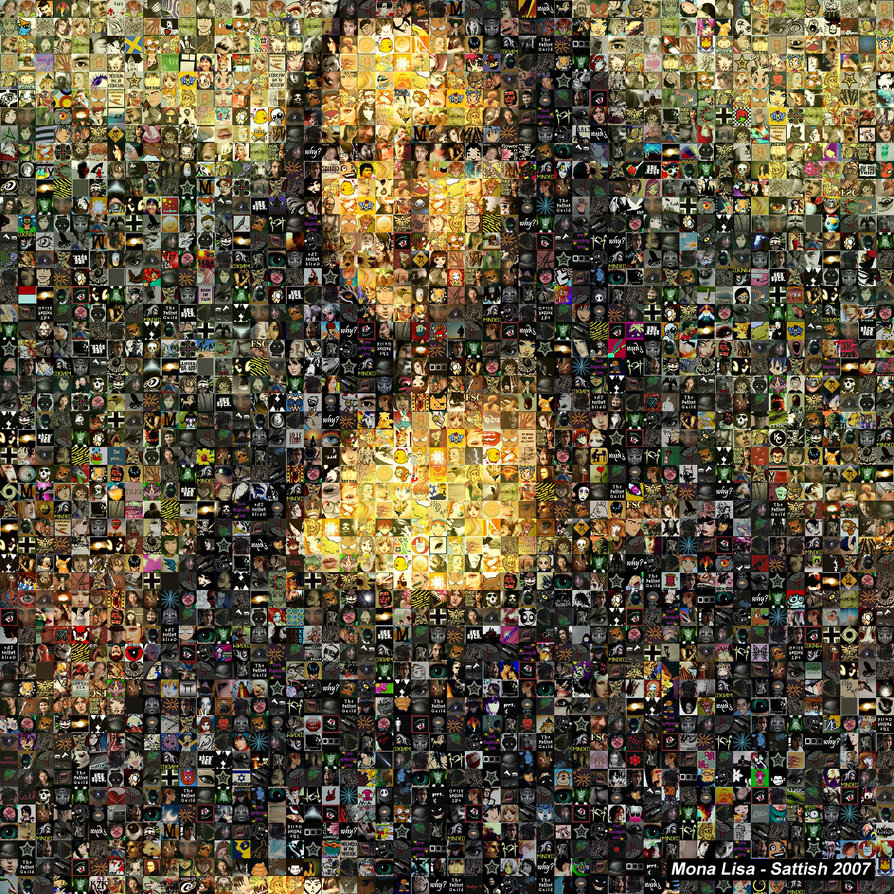
\includegraphics[width=200mm]{intro_monalisa.jpg}

\begin{abstract}

	\par Influential users are very important in the network in terms of their ability to change the distribution of the interconnections in the network. In our case, the favorite relation of the DeviantART network is investigated. Favorite relation is a interconnection between users and resources. If a user likes a resource that he views, he adds it into his list and a favorite relation is constructed. Moreover, favorite relation is so effective to increase or decrease the value of a resource in the community. If a well known user adds a resource into his list, the value of the resource increases rapidly because a lot of users follow the well known user and imitate what the well known user does and other users also add this resource into their list, by the way this resource is entered a lot of favorite lists. In this paper, an algorithm to find the most influential user respect to favorite relation is expressed. 

\end{abstract}

\tableofcontents

\chapter{Introduction}
\pagenumbering{arabic}
	
	\par \hspace{0.6cm}Networks are all around us.  Your circle of friends; the route you take to work; cars on the road; tiny neurons firing inside your brain; ecological systems.  Understanding how elements within these networks interact has fascinated scientists for decades, with pivotal results such as 6-degrees of separation, Small World Networks, to name just a few, having application to easing road congestion, enhancing computer systems and understanding human social processes. 

	\par However, all such analysis is insufficient, yet there is a need of finding the central and/or influential nodes. This project is interested in closing the gap by presenting an algorithm to find the the important nodes. Therefore, DeviantART network is chosen because DeviantART is one of the biggest networks in the online world and there is a little research on this network. 

	\par Different algorithms can be easily developed by using different heuristics but we can't sure that the developed algorithm is the desired algorithm. Therefore, we need a network for testing. After we are sure that this algorithm can find the most influential user in the network, we can run on the DeviantART network.

	\par In the first part, DeviantART is presented and its statistics are given. Then, crawled data structure and statistics are given. In the second phase, framework is introduced to use in the suggested algorithm. Details of the network generation and analysis are given. For each parameters, tests are run and results are given. In third phase, empiricial data is analyzed and parameters of the algorithm are estimated. Findings are compared to simulations and conclusion and future work are specified.

	\par Presented new method provides fascinating new directions for the development of new applications and new systems on online social networks and for a better understanding of social processes such as influence, trust and information spreading.

\chapter{DeviantART}

	\section{What is DeviantART?}

	\par \hspace{0.6cm} DeviantART is the world's largest art community where millions of artists come to share their creations to get feedback and connect with peers and mentors, etc. but it's also a hub for art enthusiasts to check out awesome artwork.

	\begin{table}[htdp]
	\begin{center}
	\textup{\Large Statistics} 
	\begin{tabular}{|p{5cm}|p{8cm}|}
	\hline
	Type & Art Display,  Social Networking\\
	\hline
	 Launch Date & 7 August, 2000\\
	\hline
	Slogan & deviantART: where art meets application! \\
	\hline
	Total Resources & 200 millions\\
	\hline
	Daily New Resources &140,000\\
	\hline
	Daily New Favorites & 1.4 million\\
	\hline
	Daily New Comments & 1.5 million\\
	\hline
	Monthly Unique Visitors & 35 millions\\
	\hline
	Monthly Page Views & 1 billion\\
	\hline
	\end{tabular}
	\end{center}
	\end{table}

	\par DeviantART is the biggest site no one's heard of with 15 million registered users becuase developers have been extremely focused on the community and building it organically - having most passionate members tell their friends, who are typically artists or sensitive to the arts in some way and so on. Users of the DeviantART are selective about who they invite to the network. Actually, this is the strength of the dA, as DeviantART has been able to build perhaps the most passionate, emotional, creative community on the web in this way.

	\clearpage

	\section{Difference of DeviantART}

	\par DeviantART isn't reallly compared to other social networks. Members specifically intend the exact submission they post in to our community. For example, at Flickr, user can \emph{dump} hundreds of photos at a time. Inherently that sets a different tone. Moreover, DeviantART accepts and encourage submissions from all mediums. At last but most importantly, DeviantART focuses on mentoring and growth and development of its members, artists. This property deviates it from Flickr, Photobucket, Facebook, Youtube, etc.

	\begin{table}[htdp]
	\begin{center}
	\textup{\Large Strong and Different Properties} 
	\begin{tabular}{|p{6.5cm}|p{6.5cm}|}
	\hline
	Chat & Scraps (Workspace)\\
	\hline
	Forum & Neighbours\\
	\hline
	Mentor & Activity Log \\
	\hline
	Tutorial & User Watch\\
	\hline
	License and Stockphoto &Submission Mediums\\
	\hline
	Journal (News) & Pandora for ART\\
	\hline
	Prints (Store) & New properties at birthday\\
	\hline
	\end{tabular}
	\end{center}
	\end{table} 

	\par There are some characters in the front of names of members in the network. These characters have some meanings, by this way you can easily find mentors for yourself.

\chapter{Crawled Data}

	\section{Category Structure}

	\par \hspace{0.6cm} There is a compherensive category structure, totally \emph{2348} categories but mainly \emph{digital art} and \emph{manga} are focused.

	\begin{itemize}
	\item Photography
	\item Digital Art
	\item Fillm Making
	\item Traditional Art
	\item Literature
	\item Flash
	\item Skins for Applications
	\end{itemize}

	\section{3D Game}

	\par \hspace{0.6cm} Since DeviantArt is too big to analyze in an one term, we must limit the analysis some categories. Therefore, we had to choose a category and we chose game art 3D because of that

	\begin{itemize}
	\item Feasible category for social analysis
	\item Narrow interest
	\item More passionate users
	\item Subcategory of the predominantly focused media of the community
	\end{itemize}

	\section{Info Structure}

	\par \hspace{0.6cm} In the DeviantArt, there are a lot of tools to socialize and get news and notifications from other artists. These tools are 

	\begin{itemize}
	\item Watcher
	\item Favorite
	\item Gallery (Prints and Scraps)
	\item Chat
	\item Forum
	\item Comment
	\item Neighbour
	\end{itemize}

	\section{Why Favorite is important?}

	\par \hspace{0.6cm} We want to find the most influential user and there are no notifications for favorite relation but if an artist follow a watcher and looks into his favorite list, this artist may be probably affected by the taste of the artist since unconsciously he is influenced by him and is interested in him favorite list when there are no notifications. Moreover, 

	\begin{itemize}
	\item Ease of use
	\item More popular
	\item Rollback option (artists can undone their favorites)
	\item Past data is available which is critical for analysis
	\end{itemize}

	\clearpage

	\section{Data Structure}

	\par \hspace{0.6cm} We have three tables, \emph{Resource, User} and \emph{Favorite} in the following design:

	\begin{table}[htdp]
	\begin{center}
	\textup{\Large Resource} 
	\begin{tabular}{|p{2cm}|p{2cm}|p{2cm}|p{2cm}|p{4cm}|}
	\hline
	ID & Name & URL & Producer & Submission Date \\
	\hline
	\end{tabular}
	\end{center}
	\end{table} 

	\begin{table}[htdp]
	\begin{center}
	\textup{\Large User} 
	\begin{tabular}{|p{2cm}|p{2cm}|p{2cm}|p{2cm}|p{4cm}|}
	\hline
	ID & Name & URL & Type & Attend Date \\
	\hline
	\end{tabular}
	\end{center}
	\end{table}

	\begin{table}[htdp]
	\begin{center}
	\textup{\Large Favorite} 
	\begin{tabular}{|p{4.25cm}|p{4.25cm}|p{4.25cm}|}
	\hline
	UserID & ResourceID & Favorite Date \\
	\hline
	\end{tabular}
	\end{center}
	\end{table}

	\large{Sets}

	\begin{itemize}
	\item $\mathcal{U} = \text{The set of the users}$
	\item $\mathcal{R} = \text{The set of the resources}$
	\item $\mathcal{F} = \text{The set of the favorites, mapping between } \mathcal{U} \text{ and } \mathcal{R}$

	\end{itemize}

	\large{Size of the sets}

	\begin{itemize}
	\item $|\mathcal{U}| = 50816$
	\item $|\mathcal{R}| = 40283$
	\item $|\mathcal{F}| = 102858$
	\end{itemize}

	\normalsize


\chapter{Framework} 

	\hspace{0.6cm}There are mainly three components to represent the DeviantART network, namely, user, resource and favorite relation. In the following pages, user will be used instead of  deviant and resource will be used instead of deviation to decrease the confusion between deviant and deviation where they are original terms that DeviantART uses.

\section{User}

	\hspace{0.6cm}User object is defined to represent the users of the DeviantART.\\
	
	There are two properties, namely, \emph{id} and \emph{authority}. 

	$$User = \{(id, authority)\}$$
	
	\emph{id} is defined to select the users uniquely and varies from 1 to the number of the users. $\mathcal{U}$ is the set of the users and U is the size of the $\mathcal{U}$.

	$$|\mathcal{U}| = U $$

	$$\mathcal{U} = \{u_{1}, u_{2}, \dots, u_{U}\}$$ 

 	\emph{authority} is to specify the influentiality of the user. \emph{authority} is a function from $\mathcal{U}$ to $[0, 1)$ and returns a value from $[0, 1)$ for each user. The more influential user is, the closer to 1 \emph{authority} is.

	$$a : \mathcal{U} \to [0, 1)$$\\	

\section{Resource}

	\hspace{0.6cm}Resource object is defined to represent the artworks (pictures, drawings, clips, etc.) in the DeviantART.\\

	There are four properties, namely, \emph{id}, \emph{quality}, \emph{favorite list}, \emph{time list}. 

	$$Resource = \{(id, quality, favorite \text{ } list,  time \text{ } list)\}$$

	\emph{id} is defined to select the resources uniquely and varies from 1 to the number of the resources. $\mathcal{R}$ is the set of the resources and R is the size of the $\mathcal{R}$.

	$$|\mathcal{R}| = R $$

	$$\mathcal{R} = \{r_{1}, r_{2}, \dots, r_{R}\}$$ 
		

 \emph{quality} is to specify the art-criticique of the artwork. \emph{quality} is a function from $\mathcal{R}$ to $[0, 1)$ and returns a value from $[0, 1)$ for each resource. The higher quality resource is, the closer to 1 \emph{quality} is. 

	$$q : \mathcal{R} \to [0, 1)$$

\emph{favorite list} holds the ids of the users that added this resource to their favorite list.

	$$|fl(r_{i})| = k \Longrightarrow fl(r_{i}) =\{u_{1}, u_{2}, \dots, u_{k}\} \text{ where } r_{i} \in \mathcal{R} \text{ and } \{u_{1}, u_{2}, .., u_{k}\}  \subseteq \mathcal{U}$$ 

$D$ is the length of the days that have passed from the start of the DeviantART to present. 

	$$|\mathcal{D}| = D$$

	$$\mathcal{D} = \{d_{1}, d_{2}, \dots, d_{D}\}$$

Corollary to \emph{favorite list, time list} holds the days when these users added the resource. If a user added the resource before than others, his index will be smaller than others.

	$$|tl(r_{i})| = k \Longrightarrow tl(r_{i}) =\{d_{1}, d_{2}, .., d_{k}\} \text{ where } r_{i} \in \mathcal{R} \text{ and } d_{1} \le d_{2} \dots \le d_{k-1} \le d_{k} \le D\}$$ 

	$$|fl{r_{i}}| = |tl(r_{i})| \text{ must hold since they are respective lists of each other}$$

\clearpage

\section{Network} 

	\hspace{0.6cm}Network object is defined to represent favorite relation between users and resources in the DeviantART. Favorite relation maps users onto resources so each user chooses a subset of the resources set. \\

	$$Favorite = \{user, resource, day\}$$

	$$ \mathcal{F} = \{f(u_{i}, r_{j}, d_{k}) | u_{i} \in \mathcal{U}, r_{j} \in \mathcal{R}, d_{k} \in \mathcal{D}\}$$ \\

	We can imagine favorite relation ($\mathcal{F}$) as a bipartite matching where users and resources are nodes and adding into favorite list is the edge because there are two partitions composed of user ($\mathcal{U}$) and resource ($\mathcal{R}$) sets and there will be a link between partitions, not inside the partitions since users can add resources but can't follow the other users since we are just interested in favorite relation or resources can't be linked with other resources . Therefore, there will be an edge $f_{ijk}$ only if $u_{i}$ adds the $r_{j}$ into his list on the day $d_{k}$. \\

\chapter{Data Generation}

\section{Assumptions}

	\begin{itemize}
	\item All users and resources are available in whole simulation time.
	\item Despite quality values are changeable, authority values are permanent.
	\item Quality values of resources and Authority values of users are generated according to Power laws.
	\item Favorite relation can be done one time and cannot be deleted or updated.
	\item Network needs some time to respond updates, setup window
	\end{itemize}

\section{Distributions of the Generation}

	\hspace{0.6cm}We definitely need a probability distribution to generate \emph{authority} values of the users and \emph{quality} values of the resources. Since a lot of users should have low \emph{authority} values and a lot of resources should have low \emph{quality} values, we need sharply decreasing probability distributions. Therefore, we chose two distributions: $2 - 2x$ and the family of $\frac{1}{x^n}$ where $n\ge 1$ and $x \in [0, 1)$. The first distribution is a real probability distribution but second one isn't since \\

	$$\int_{-\infty}^{\infty} \!  (2-2x)\, dx = 1$$ \\

	$$\int_{-\infty}^{\infty} \! \frac{1}{x^n}\, dx \not= 1$$ \\

	Therefore, there is a check while generating random stream with these distributions. If generated random number isn't in $[0, 1)$, repeat the procedure to get a number in the range. \\

	Inverse transform method is used to generate random variates from these distributions.

	Random variate calculation of the $(2-2x)$ distribution:
	\begin{eqnarray*}
		 \int_{-\infty}^x \!  (2-2x)\, dx  = 2x -  x^2  & = & y \text{ where } y \in [0, 1) \text{ is a random number}\\
		x^2-2x+1 & = & 1 - y \\
		(x-1)^2 & = & 1 - y \\
		x - 1 & = & -\sqrt (1 - y) \\
		x & = & 1 - \sqrt(1-y)
	\end{eqnarray*}

	Since $y$ is randomly distributed, $1-y$ is also randomly distributed so we can use $y$ instead of $1-y$ and generator formula becomes 

	$$1-\sqrt y  \text{ where } y \text{ is a random number}$$ \\
		
	Random variate calculation of the family of the $(\frac{1}{x^n})$ distribution:
	\begin{eqnarray*}
		 \int_{-\infty}^x \!  (\frac{1}{x})\, dx  = \ln x & = & y \text{ where } y \in [0, 1) \text{ is a random number and } n = 1\\
		x & = & e^y \\
	\end{eqnarray*}

	However, by this formula we can calculate numbers which are outside of the range \\

	$$x \not\in [0, 1)$$ \\

	since the distribution isn't a probability distribution. We can check the generated values and take the values that are in the range but this is also so costly.\\

	Therefore, we thought about using minus logarithm of the random numbers to simulate the distribution and by dividing with $n$, whole family can be represented. \\

	Generator formula becomes\\
	
	$$\frac{-\log y}{n} \text{ where } y \text{ is a random number and } n \ge 1 $$

	Moreover, we yet need to check each generated variate since this can also generate variates outside the range $[0, 1)$ but the probability of this is much smaller than the previous generator.

	While $n$ is increasing, the mean of the distribution decreases to zero which means that  a lot of users have small \emph{authority} values and have a minor effect on the network.

	$$\lim_{n \to +\infty} \frac{-\log y}{n} = 0 $$

	\clearpage

\section{Generation of the Users}

	\hspace{0.6cm}\emph{id} property is incremented by one in each user generation. The value of the \emph{authority} property is generated by the chosen distribution function.

	$$u_{i} = \{(i, a_{i})| 1 \le i \le U, a_{i} \in [0,1) \} $$  

\section{Generation of the Resources}

	\hspace{0.6cm}\emph{id} property is incremented by one in each resource generation. The value of the \emph{quality} property is generated by the chosen distribution function.

	$$r_{i} = \{(i, q_{i})| 1 \le i \le R, q_{i} \in [0,1) \} $$  

\section{Matching of Deviants and Deviations}	
	
	\hspace{0.6cm}We have users and resources

	\begin{eqnarray*}
	\mathcal{U} = \{u_{i}|1 \le i \le U\}\\
	\mathcal{R} = \{r_{i}|1 \le i \le R\}
	\end{eqnarray*}

	By matching these two partitions we get favorite relation. 

	$$\mathcal{F} = \{f_{ijk} : (u_{i}, r_{j}, d_{k})| u_{i} \in \mathcal{U}, r_{j} \in \mathcal{R}, d_{k} \in \mathcal {D}\} $$

\clearpage

	\large{Matching algorithm:} 
	
	\begin{equation}
	 \hspace{-6cm}\text{For } d  =  1  \text{ to } D  
	\end{equation}

	\begin{equation}
   	\hspace{-4cm}t_{max}  \leftarrow  \mathcal{N}(\mu, \sigma^2) 
	\end{equation}	

	\begin{equation}	
	\hspace{-4cm}\text{For } t=1 \text{ to } t_{max} 		
	\end{equation}
	
	\begin{eqnarray}	
	&\hspace{-2.2cm}u_{i} \leftarrow \text{Uniform}[1, U] \nonumber \\
	&\hspace{-2.2cm}r_{j} \leftarrow \text{Uniform}[1, R]  		
	\end{eqnarray}	

	\begin{equation}
	\hspace{1cm}\text{if } f(u_{i}, r_{j}, d_{k}) \not \in \mathcal{F} \text{ where }\exists d_{k} \in \mathcal{D}
	\end{equation}

	\begin{eqnarray}	
	\hspace{2.8cm}fl(r_{j}) & = &fl(r_{j}) \cup u_{i} \nonumber \\
	tl(r_{j}) &=& tl(r_{j}) \cup d \nonumber \\
           f(u_{i}, r_{j}, d) &\in &\mathcal{F} \text{ with } \mathcal{P}(q(r_{j}))		
	\end{eqnarray}

	\begin{eqnarray}	
	\hspace{3.5cm}fl(r_{j}) &= &fl(r_{j}) \nonumber \\
	tl(r_{j}) & = &  tl(r_{j}) \nonumber \\
           f(u_{i}, r_{j}, d) &\not \in &\mathcal{F} \text{ with } 1-\mathcal{P}(q(r_{j}))		
	\end{eqnarray}

	\begin{equation}	
	\hspace{4.7cm}q(r_{j})= \max \{q(r_{j}, a(u_{i})) \} \text{ if }{ f(u_{i}, r_{j}, d) \in \mathcal{F}}  
	\end{equation}

	\hspace{3.2cm}end\\

	\hspace{2.4cm}end\\

	\hspace{1.6cm}end\\

	\clearpage
	
	\normalsize
	There are \emph{three} parameters used in the data generation, namely, \emph{simulation length} ($D$),  $\alpha$ and $\beta$. \emph{simulation length} is self descriptive and is used to specify the number of the days to generate matching data.  \par
	We call a \emph{transaction} that a user looks a resource and whether s/he adds it into her/his \emph{favorite} list and denoted by $t$. $\alpha$ is used to calculate the mean ($\mu$) of the normal distribution which is used to generate the number of daily transactions ($t_{max}$). $\beta$ is used to scale the mean ($\mu$) which is calculated by using $\alpha$, to calculate the variance ($\sigma^2$) of the normal distribution and the calculated $\mu$ and $\sigma^2$ are used in the equation ($3.2$). The details of calculation of each as follows: \\

	\begin{equation}
	\mu = \alpha \times U \times R
	\end{equation}
	\begin{equation}
	\sigma^2 =  \beta * \mu 
	\end{equation}
	Here are the step by step procedure explained: 

\begin{itemize}

\item Calculate the mean ($\mu$) of the normal distribution which is used to generate the number of daily transactions by the equation ($3.8$).

\item Calculate the variance ($\sigma^2$) of the normal distribution which is used to generate the number of daily transactions by the equation ($3.9$).

\item Create a pseudo variate generator for the normal distribution with parameters $\mu$ and $\sigma^2$.

\item Set the simulation day to one

\item Repeat as much as \emph{simulation length} ($D$) - equation ($3.1$)

	\begin{itemize}

	\item Generate a number for daily transactions ($t_{max}$) - equation($3.2$)

	\item Repeat as much as $t_{max}$ - equation ($3.3$)

		\begin{itemize}

		\item Randomly choose a user $u_{i}$ - equation($3.4$)

		\item Randomly choose a resource $r_{j}$ - equation($3.4$) 

		\item Check the \emph{favorite list} ($fl(r_{j})$) of the resource $r_{j}$ for the chosen user ($u_{i}$) - equation ($3.5$)

		\item If chosen user $u_{i}$ has already added the chosen resource $r_{j}$ into her/his list, there is no action and continue for new transaction $t$. In other words, the {favorite list} of the resource ($fl(r_{j})$)  already contains the randomly chosen deviant - equation($3.5$) is false

		\item Else equation ($3.5$) is true and user $u_{i}$ hasn't added the chosen resource $r_{j}$ yet, so give a chance to user to add the resource into his list. User $u_{i}$ adds the resource $r_{j}$ into his list with a propability proportional to its quality ($q(r_{j})$) - equation ($3.6$) and ($3.7$)

		\item If chosen user $u_{i}$ adds the chosen resource into his list by equation ($3.6$), update the \emph{quality} of the resource ($r_{j}$) - equation ($3.8$). If influential users add the resource into their list, the \emph{quality} of the resource ($q(r_{j})$) increases and so the probability increases so that other users can add the resource  $r_{j}$ when they meet the resource $r_{j}$

		\end{itemize}

	\end{itemize}

\end{itemize}	

\chapter{Analysis of the Generated Data}

	\section{Algorithm}

	\hspace{0.6cm} We have explained how to generate data, now we will explain the how to analyze the data. Analysis phase doesn't know the internal dynamics of the generated data but since we know true values, we can easily check their correctness and the power of the algorithm.

	\hspace{0.6cm}Firstly, create a \emph{map} because at the end of anaysis this data structure will be filled. This data structure holds a flag for each user-resource pair and this number specifies whether this user is the most influential user for the resource. Therefore, we can define this data structure a function from users and resources to $\{0,1\}$ since a user is the most influential user or not.

	$$h : \mathcal{U} \times \mathcal{R} \rightarrow \{0, 1\}$$

	$$ \mathcal{H} = \{h(u_{i}, r_{j})| u_{i} \in \mathcal{U}, r_{j} \in \mathcal{R}\}$$
	
	$$hsum(u_{i}) = \sum_{j=1}^R h(u_{i}, r_{j})$$

	$$vsum(u_{i}) = \sum_{j=1}^R \sum_{k=1}^D f(u_{i}, r_{j}, d_{k}) $$

	The bigger $hsum(u_{i})$ is, the more influential user $u_{i}$ may be. After scaling with the size \emph{favorite list} of resources and the number of resources that users has added their list, the distribution of $h(u_{i})$s is correlated with the distribution that is used to generate the users.

	

	Frequency list of a resource is the distribution of the numbers of the users that have added this resource into their list. Therefore, frequency list can be represented as a function from the days of the data to the number of users since at most all users can add the resource in a day.

	$$freq : [1, D] \rightarrow [0, U]$$

	\begin{equation}
	freq(r_{j}, k) = \sum_{i=1}^U f(u_{i}, r_{j}, d_{k}) \text{ where } 1 \le k \le D \nonumber
	\end{equation}

	\begin{equation}
	freqList(r_{i}) = \{freq(r_{i}, k)| 1\le k \le D\} \nonumber
	\end{equation}

	Moreover, we have two more parameters, namely, \emph{derivation window} and \emph{setup window}. The sizes of these windows are effected by the length of the data and daily transactions. Therefore, these window sizes must be chosen while taking consideration the length ($D$) and the average of the daily transactions ($\mu$). Since we can calculate  $\mu$ and $D$ in real data, we can easily agree on the window sizes.

	\begin{eqnarray*}
	dw & \leftarrow & derivation \text{ } window \\
	sw & \leftarrow & setup \text{ } window
	\end{eqnarray*}

	\clearpage 
	
	\text{The algorithm to find the most influential user:}
	\begin{eqnarray*}
	&\hspace{-14.4cm}\text{Foreach } r_{j} \in \mathcal{R} \nonumber\\
	&\hspace{-11.9cm}p(r_{j}) = 0, inc(r_{j}) = 0 \\
	&\hspace{-12.1cm}\text{for } k = 1 \text{ to } D-dw \\
           &\hspace{1cm}p(r_{j}) \text{ }  = k \text{ if } 
	\begin{cases}	
p(r_{j}) \le \sum_{i=k}^{k+dw} freq(r_{j}, i) \\ freq(r_{j}, p(r_{j}))-freq(r_{j}, p(r_{j})-1) \le freq(r_{j}, k) - freq(r_{j}, k-1)\\
	\end{cases}\\
	&\hspace{-10.9cm}\text{for } k = p(r_{j}-sw) \text{ to } p(r_{j})\\
	&\hspace{-1.1cm}\mathcal{H} = \mathcal{H} \cup \{h(fl(r_{j})[m], r_{j})= 1 \} \text{ where } tl(r_{j})[m] = p(r_{j}), 0 \le m \le |fl(r_{j})|\\
	&\hspace{-14.6cm}\text{endfor} \\
	&\hspace{-15.2cm}\text{endforeach} \\
	&\hspace{-11.4cm}maxList = \max\{fl(r_{j})| r_{j} \in \mathcal{R}\} \\
	&\hspace{-14.5cm}\text{for } i = 1 \text{ to } U \\
	&\hspace{-13.1cm}\text{for } j = 1 \text{ to } R \\
	&\hspace{-10.1cm}h(u_{i}, r_{j}) = \frac{h(u_{i}, r_{j}) \times fl(r_{j})}{maxList} \\
	&\hspace{-14.6cm}\text{endfor} \\
	&\hspace{-15.9cm}\text{endfor} \\
	&\hspace{-10.2cm}u_{influential} = max\{\frac{hsum(u_{i})}{vsum(u_{i})}| 1 \le i \le U\}
	\end{eqnarray*}

	\clearpage
	
	\section{Parameter Analysis}

	\begin{itemize}

	\item \textbf{User Distribution Analysis}

\begin{center}
\textup{\textbf{$U=1,000; R=10,000; D=1,000; dw=15; sw=15; \alpha=0.005; \beta=2; 12\text{ }Resource\text{ }Distribution; 100\text{ }Runs$\\}}
\textup{\\}
\begin{tabular}{|c|c|c|c|}
\hline
\textbf{$n$} & \textbf{$\mu_{real}$} & \textbf{$\mu_{estimated}$} & \textbf{$\Delta$}\\
\hline
0 & 0.9713 & 0.8285 & 0.1428 \\
\hline
2 & 0.9966 & 0.6147 & 0.3819 \\
\hline
4 & 0.9876 & 0.9061 & 0.0814 \\
\hline
6 & 0.9503 & 0.9474 & 0.0029 \\
\hline
8 & 0.8540 & 0.8491 & 0.0049 \\
\hline
10 & 0.7374 & 0.7363 & 0.0010 \\
\hline
\end{tabular}
\end{center}

	\item \textbf{Resource Distribution Analysis}

\begin{center}
\textup{\textbf{$U=1,000; R=10,000; D=1,000; dw=15; sw=15; \alpha=0.005; \beta=2; 12\text{ }User\text{ }Distribution; 500\text{ }Runs$\\}}
\textup{\\}
\begin{tabular}{|c|c|c|c|}
\hline
\textbf{$n$} & \textbf{$\mu_{real}$} & \textbf{$\mu_{estimated}$} & \textbf{$\Delta$}\\
\hline
0 & 0.6213 & 0.6205 & 0.0008 \\
\hline
2 & 0.6301 & 0.6288 & 0.0013 \\
\hline
4 & 0.6303 & 0.6300 & 0.0003 \\
\hline
6 & 0.6161 & 0.6155 & 0.0006 \\
\hline
8 & 0.6310 & 0.6308 & 0.0002 \\
\hline
10 & 0.6308 & 0.6300 & 0.0008 \\
\hline
\end{tabular}
\end{center}

	\item \textbf{Derivation and Setup Window Analysis}

\begin{center}
\textup{\textbf{$U=1,000; R=10,000; D=1,000; \alpha=0.005; \beta=2; 10\text{ }Resource\text{ }and\text{ }User\text{ }Distribution, 100\text{ }Runs$\\}}
\textup{\\}
\begin{tabular}{|c|c|c|c|}
\hline
\textbf{$dw-sw$} & \textbf{$\mu_{real}$} & \textbf{$\mu_{estimated}$} & \textbf{$\Delta$}\\
\hline
1 & 0.7274 & 0.6483 & 0.0791 \\
\hline
2 & 0.7326 & 0.7204 & 0.122 \\
\hline
3 & 0.7405 & 0.7324 & 0.0081 \\
\hline
4 & 0.7236 & 0.7210 & 0.0025 \\
\hline
6 & 0.7201 & 0.7172 & 0.0029 \\
\hline
8 & 0.7216 & 0.7154 & 0.0061 \\
\hline
\end{tabular}
\end{center}

	\item \textbf{Simulation Length Analysis}

\begin{center}
\textup{\textbf{$U=1,000; R=10,000; dw=10; sw=10; \alpha=0.005; \beta=2; 8\text{ }Resource\text{ }and\text{ }User\text{ }Distribution; 100\text{ }Runs$\\}}
\textup{\\}
\begin{tabular}{|c|c|c|c|}
\hline
\textbf{$D$} & \textbf{$\mu_{real}$} & \textbf{$\mu_{estimated}$} & \textbf{$\Delta$}\\
\hline
100 & 0.8665 & 0.8640 & 0.0025 \\
\hline
200 & 0.8588 & 0.8575  & 0.0014 \\
\hline
300 & 0.8529 & 0.8518  & 0.0011 \\
\hline
400 & 0.8395 & 0.8303 & 0.0092 \\
\hline
600 & 0.8465 & 0.8454 & 0.0011 \\
\hline
800 & 0.8623 & 0.8607 & 0.0016 \\
\hline
\end{tabular}
\end{center}


	\item \textbf{Number of Resources and Daily Transactions Analysis}

\begin{center}
\textup{\textbf{$U=1,000; D=500; dw=10; sw=10; \alpha=0.005; \beta=2; 8\text{ }Resource\text{ }and\text{ }User\text{ }Distribution; 100\text{ }Runs$\\}}
\textup{\\}
\begin{tabular}{|c|c|c|c|}
\hline
\textbf{$R$} & \textbf{$\mu_{real}$} & \textbf{$\mu_{estimated}$} & \textbf{$\Delta$}\\
\hline
300 & 0.8623 & 0.5774 & 0.2848 \\
\hline
625 & 0.8489 & 0.7309 & 0.1181 \\
\hline
1250 & 0.8672 & 0.8287 & 0.0385 \\
\hline
2500 & 0.8470 & 0.8356 & 0.0114\\
\hline
5000 & 0.8547 & 0.8464 & 0.0083\\
\hline
\end{tabular}
\end{center}

	\item \textbf{Daily Transactions Analysis}

\begin{center}
\textup{\textbf{$U = 1,000; R = 2,000; D = 500; dw=10; sw=10; \beta=2; 8 \text{ }Resource \text{ }and \text{ }User\text{ } Distribution; 100\text{ }Runs$\\}}
\textup{\\}
\begin{tabular}{|c|c|c|c|}
\hline
\textbf{$\alpha\text{ }(t_{max})$} & \textbf{$\mu_{real}$} & \textbf{$\mu_{estimated}$} & \textbf{$\Delta$}\\
\hline
0.001 (2) & 0.8627 & 0.8053 & 0.0574 \\
\hline
0.002 (4) & 0.8603 & 0.8482 & 0.0122 \\
\hline
0.0025 (5) & 0.8519 & 0.8444 & 0.0075 \\
\hline
0.005 (10) & 0.8555 & 0.8351 & 0.0204 \\
\hline
0.01 (20) & 0.8438 & 0.8016 & 0.0422 \\
\hline
0.02 (40) & 0.8645 & 0.7401 & 0.1244 \\
\hline
0.025 (50) & 0.8569 & 0.6786 & 0.1783 \\
\hline
0.05 (100) & 0.8671 & 0.4177 & 0.4494 \\
\hline
\end{tabular}
\end{center}

	\end{itemize}
\clearpage

	\begin{itemize}

	\item \textbf{Summary:}

		\begin{itemize}

		\item User Distribution is the most important parameter in the simulation. When the mean of the authority values of the most effective users goes down, algorithm gives better results.

		\item When User Distribution is selected carefully, actually sufficiently small, artwork distribution doesn't matter.

		\item The sizes of the derivation and setup windows behave in a bell curve so these window sizes should be chosen by the analysis and should be sufficiently large, not so much because then results worsen.

		\item The longer simulation length  is, the better results are found. Therefore,  simulation length must be long as much as possible.

		\item The number of daily transactions is also important and also follows a bell curve and there is an optimum value to be determined. 

		\end{itemize}

	\end{itemize}

\chapter{Analysis of Empiricial Data}

	\section{Power Law at Everywhere}

	\subsection{User}

	There are three power laws in the user analysis.

	\begin{itemize}
	\item Produce List Size Distribution $\gamma = 4.08$ (Figure7.1)
	\item Favorite List Size Distribution $\gamma = 1.71$ (Figure7.2)
	\item Inter Favorite Time Distribution $\gamma = 3.86$ (Figure7.3)
	\end{itemize}
	
	\vspace{5cm}
	\begin{figure}
	\hspace{-3.7cm}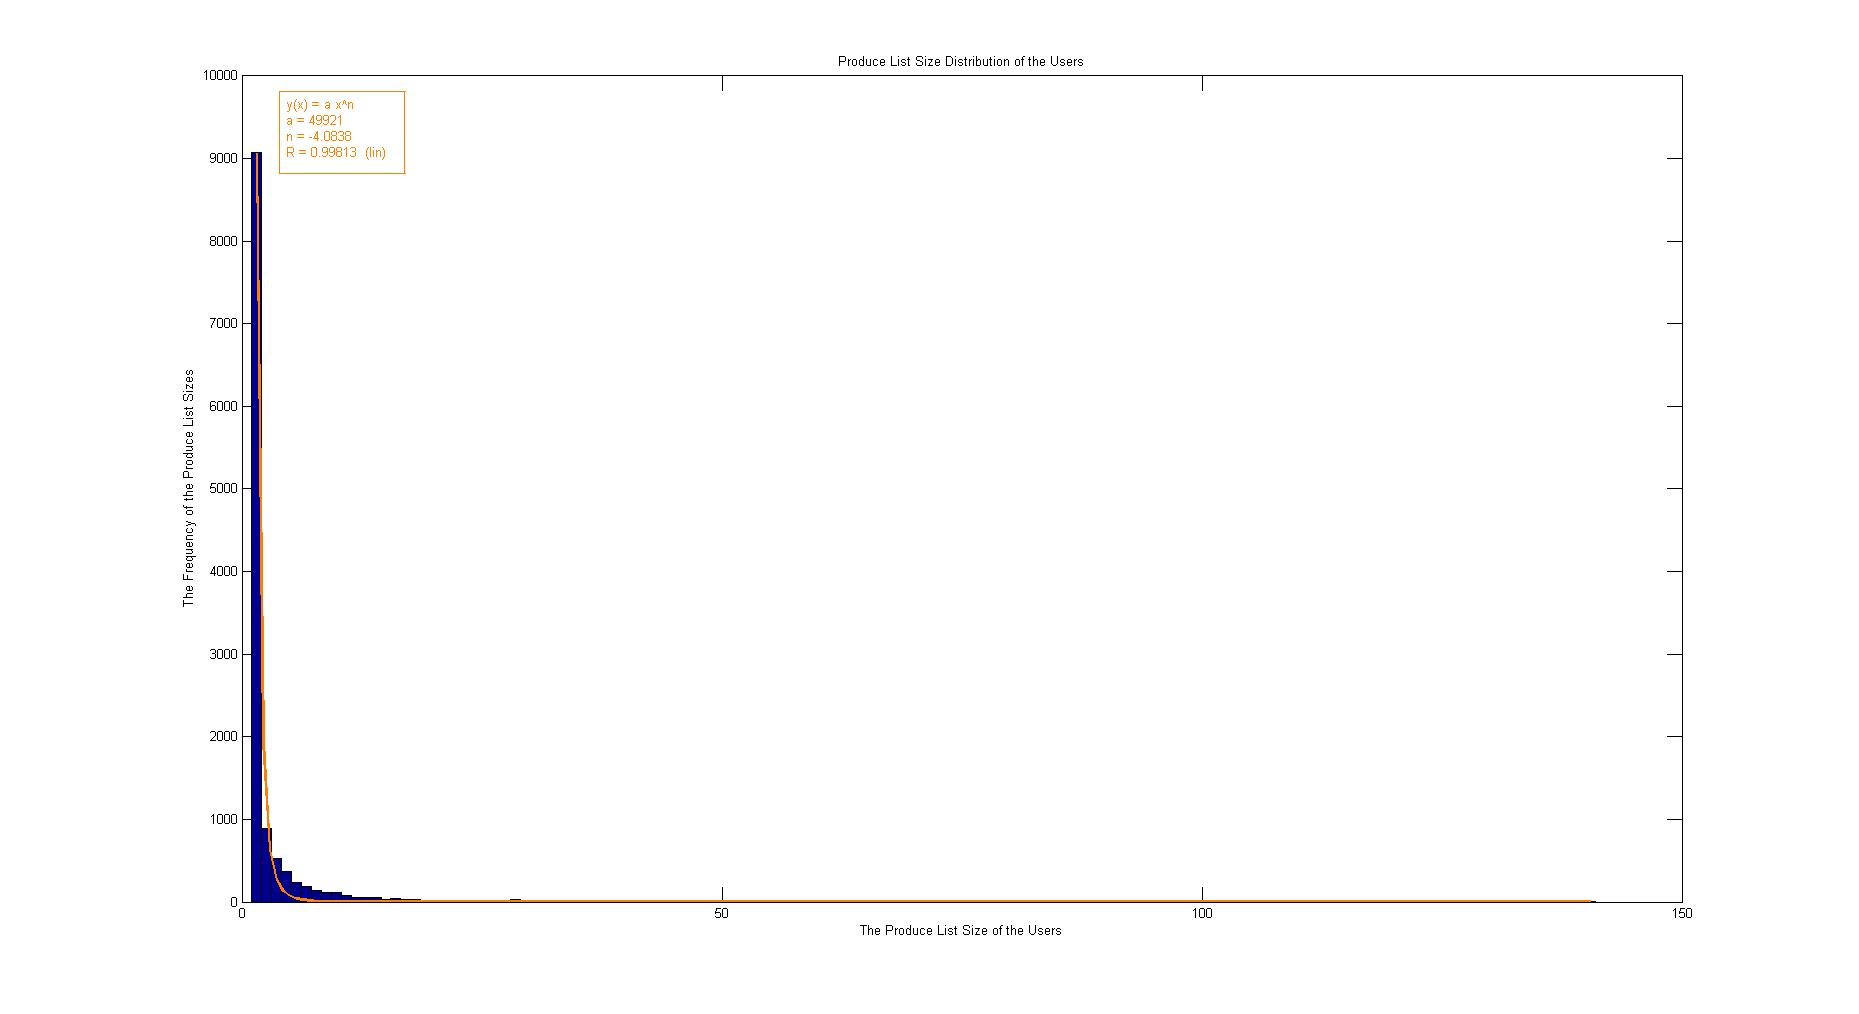
\includegraphics[width=200mm]{userProdDist.jpg}
	\caption{Produce List Size Distribution}
	\end{figure}

	\vspace{5cm}
	\begin{figure}
	\hspace{-3.7cm}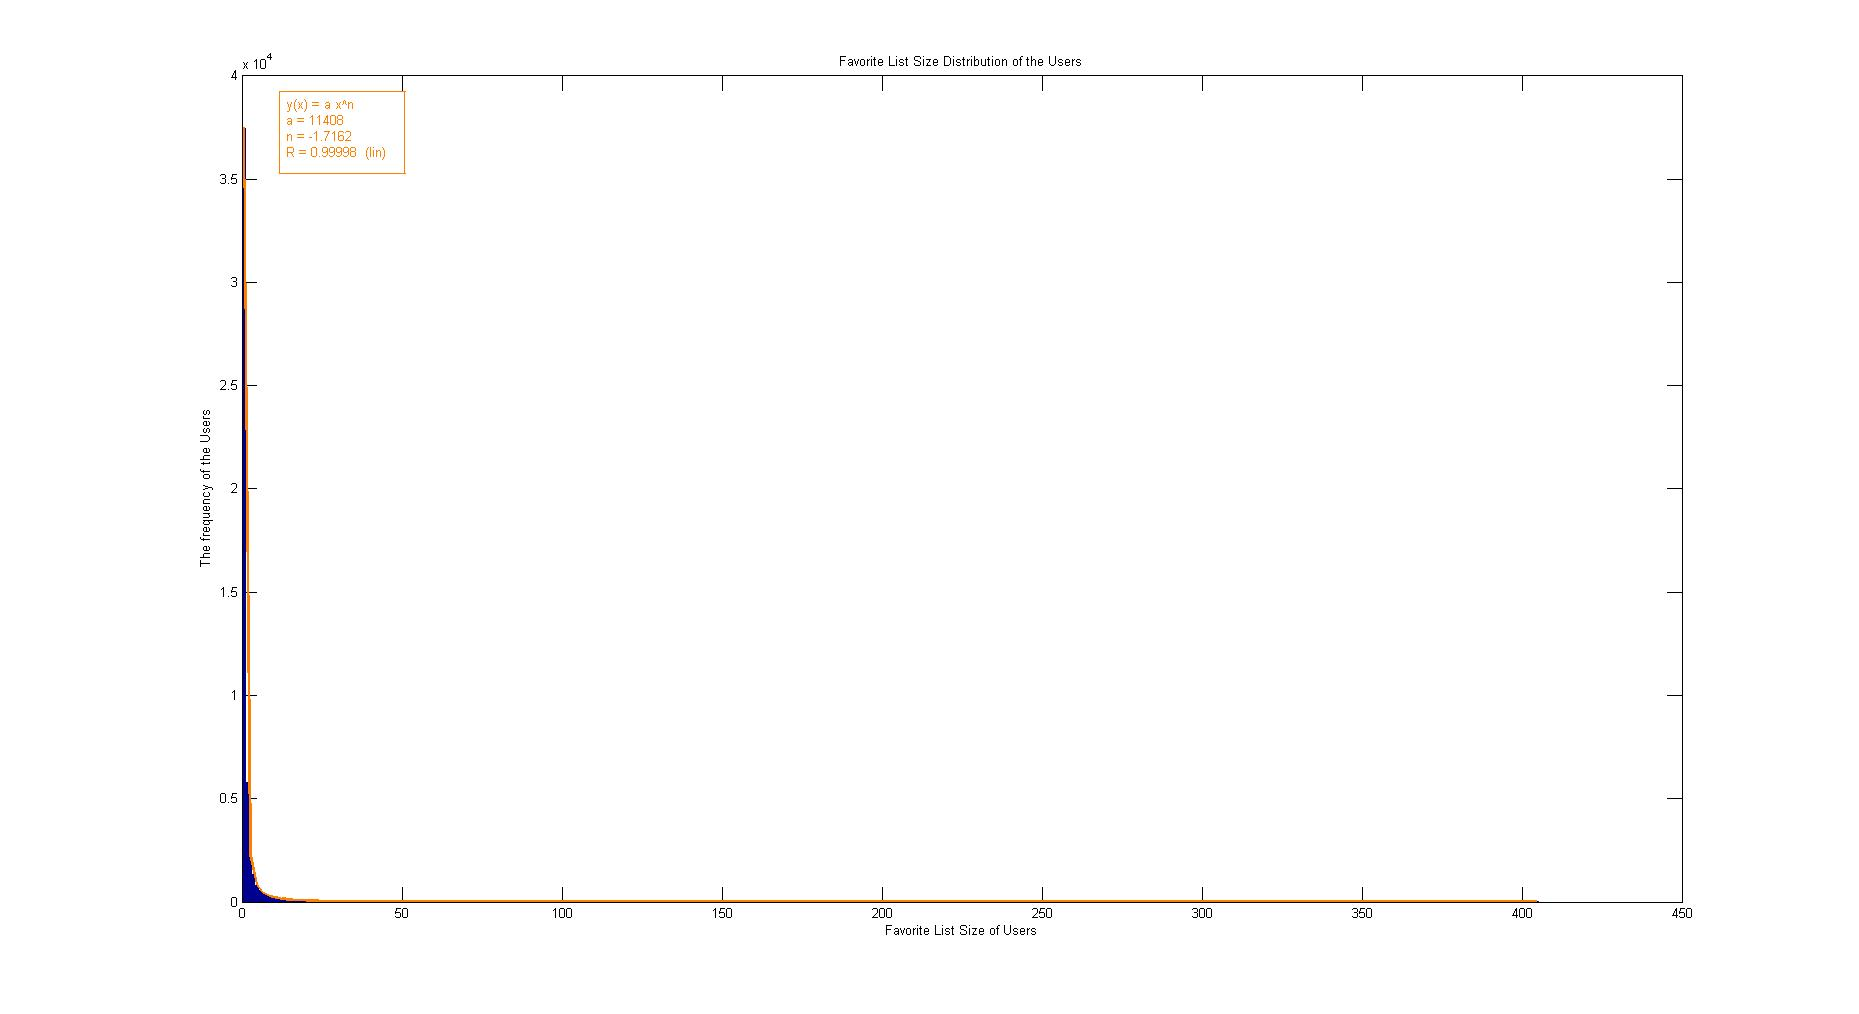
\includegraphics[width=200mm]{userFavDist.jpg}
	\caption{Favorite List Size Distribution}
	\end{figure}

	\vspace{5cm}
	\begin{figure}
	\hspace{-3.7cm}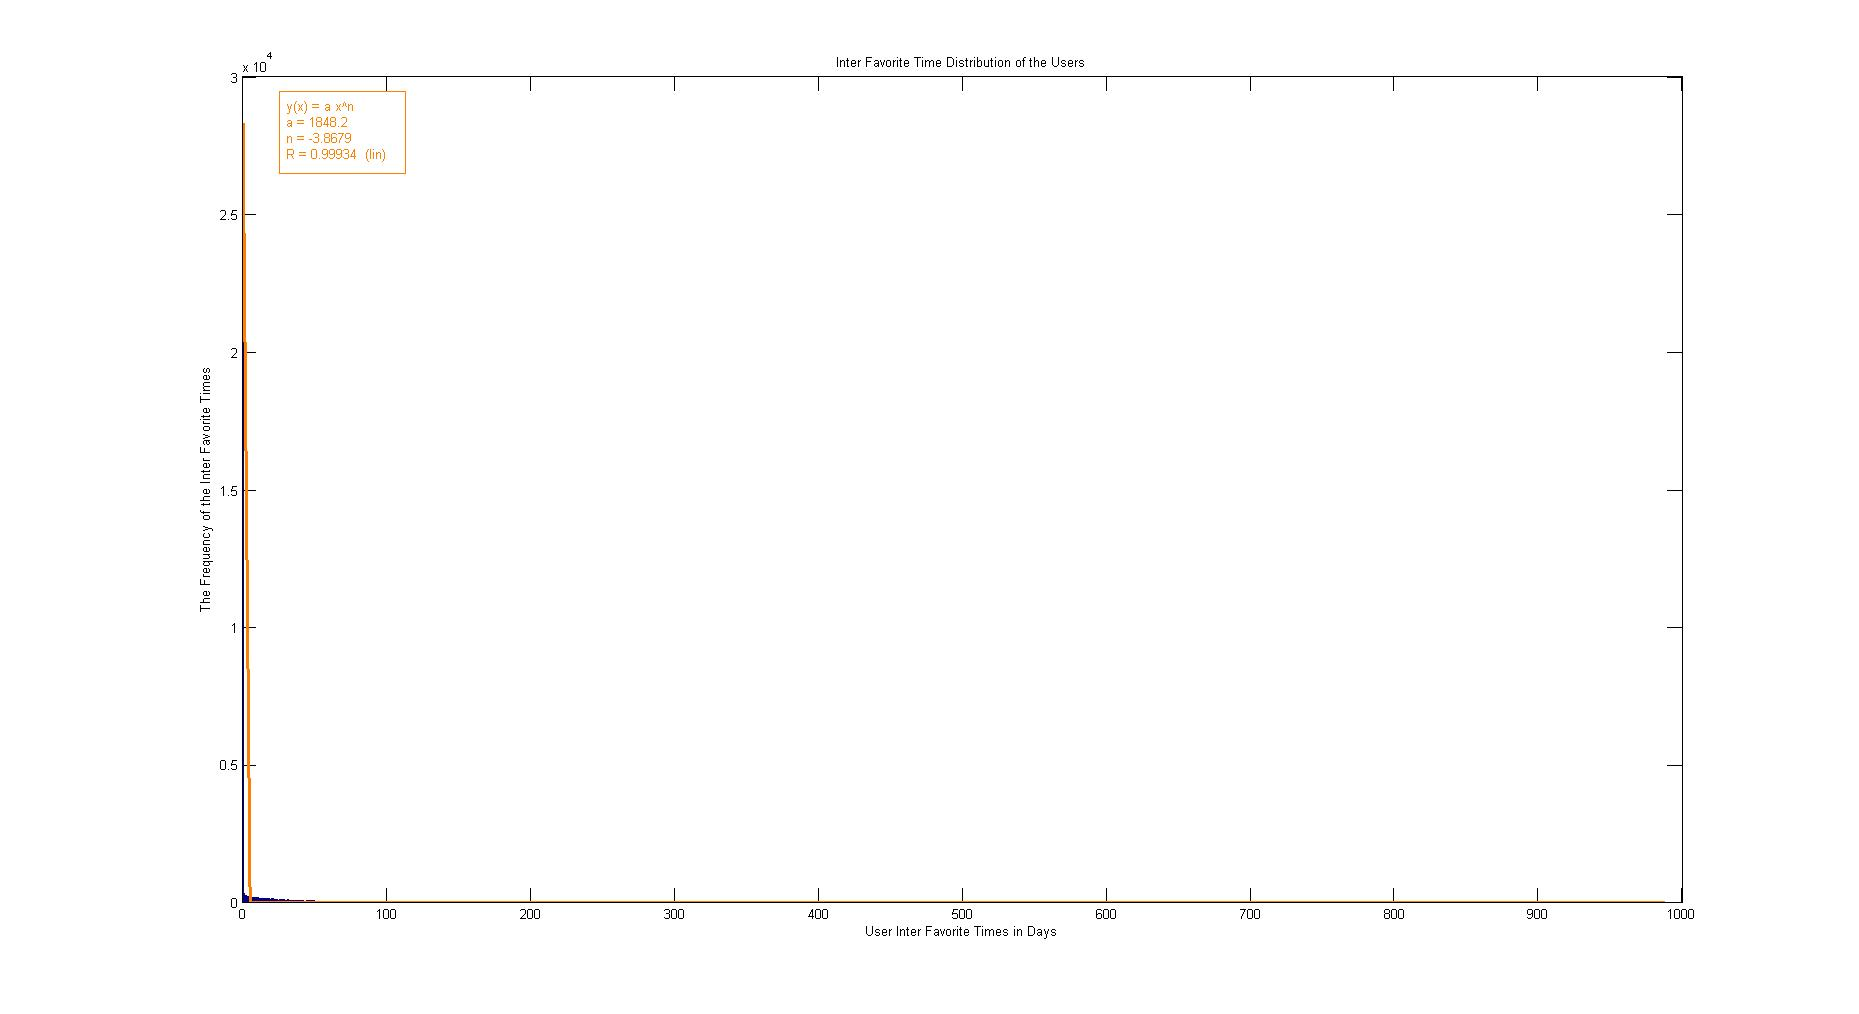
\includegraphics[width=200mm]{userInterDist.jpg}
	\caption{Inter Favorite Time Distribution}	
	\end{figure}

	\clearpage

	\subsection{Resource}

	There are two power laws in the resource analysis.

	\begin{itemize}
	\item Favorite List Size Distribution $\gamma = 1.6$ (Figure 7.4)
	\item Inter Favorite Time Distribution $\gamma = 2.14$ (Figure7.5)
	\end{itemize}

	\vspace{5cm}
	\begin{figure}
	\hspace{-3.7cm}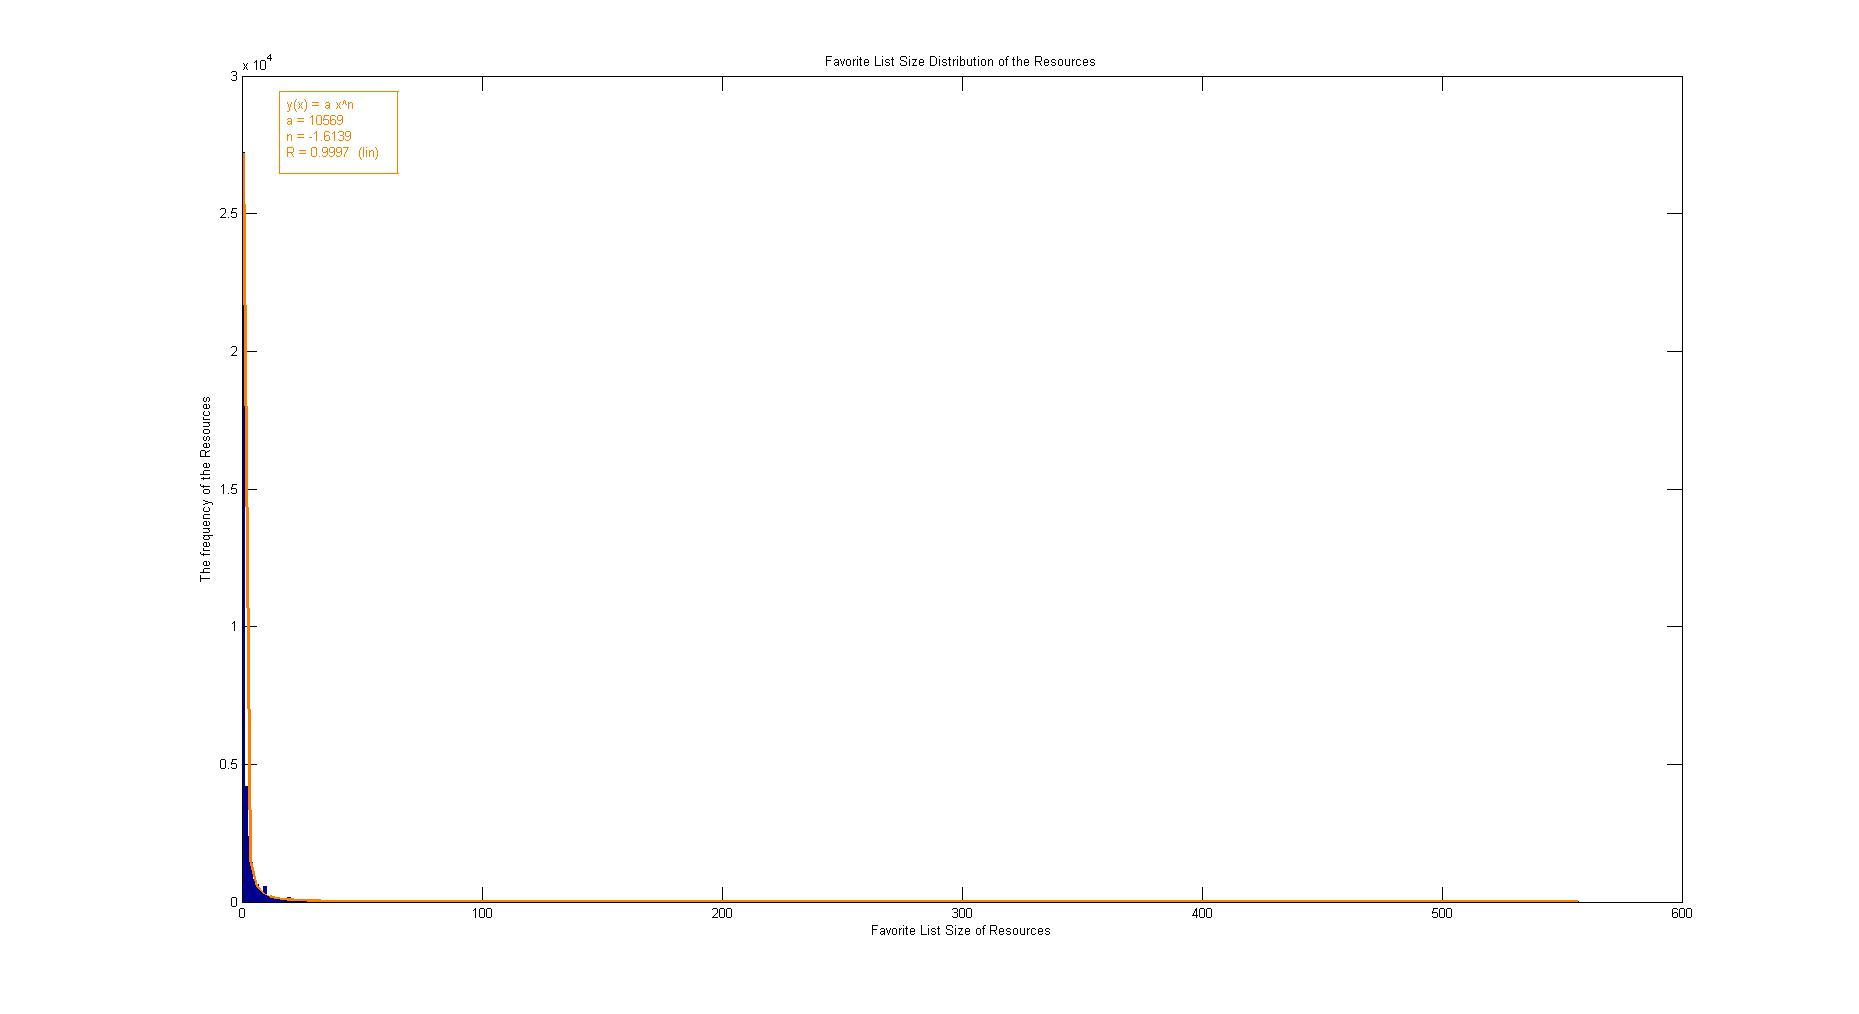
\includegraphics[width=200mm]{resFavDist.jpg}
	\caption{Favorite List Size Distribution}
	\end{figure}

	\vspace{5cm}
	\begin{figure}
	\hspace{-3.7cm}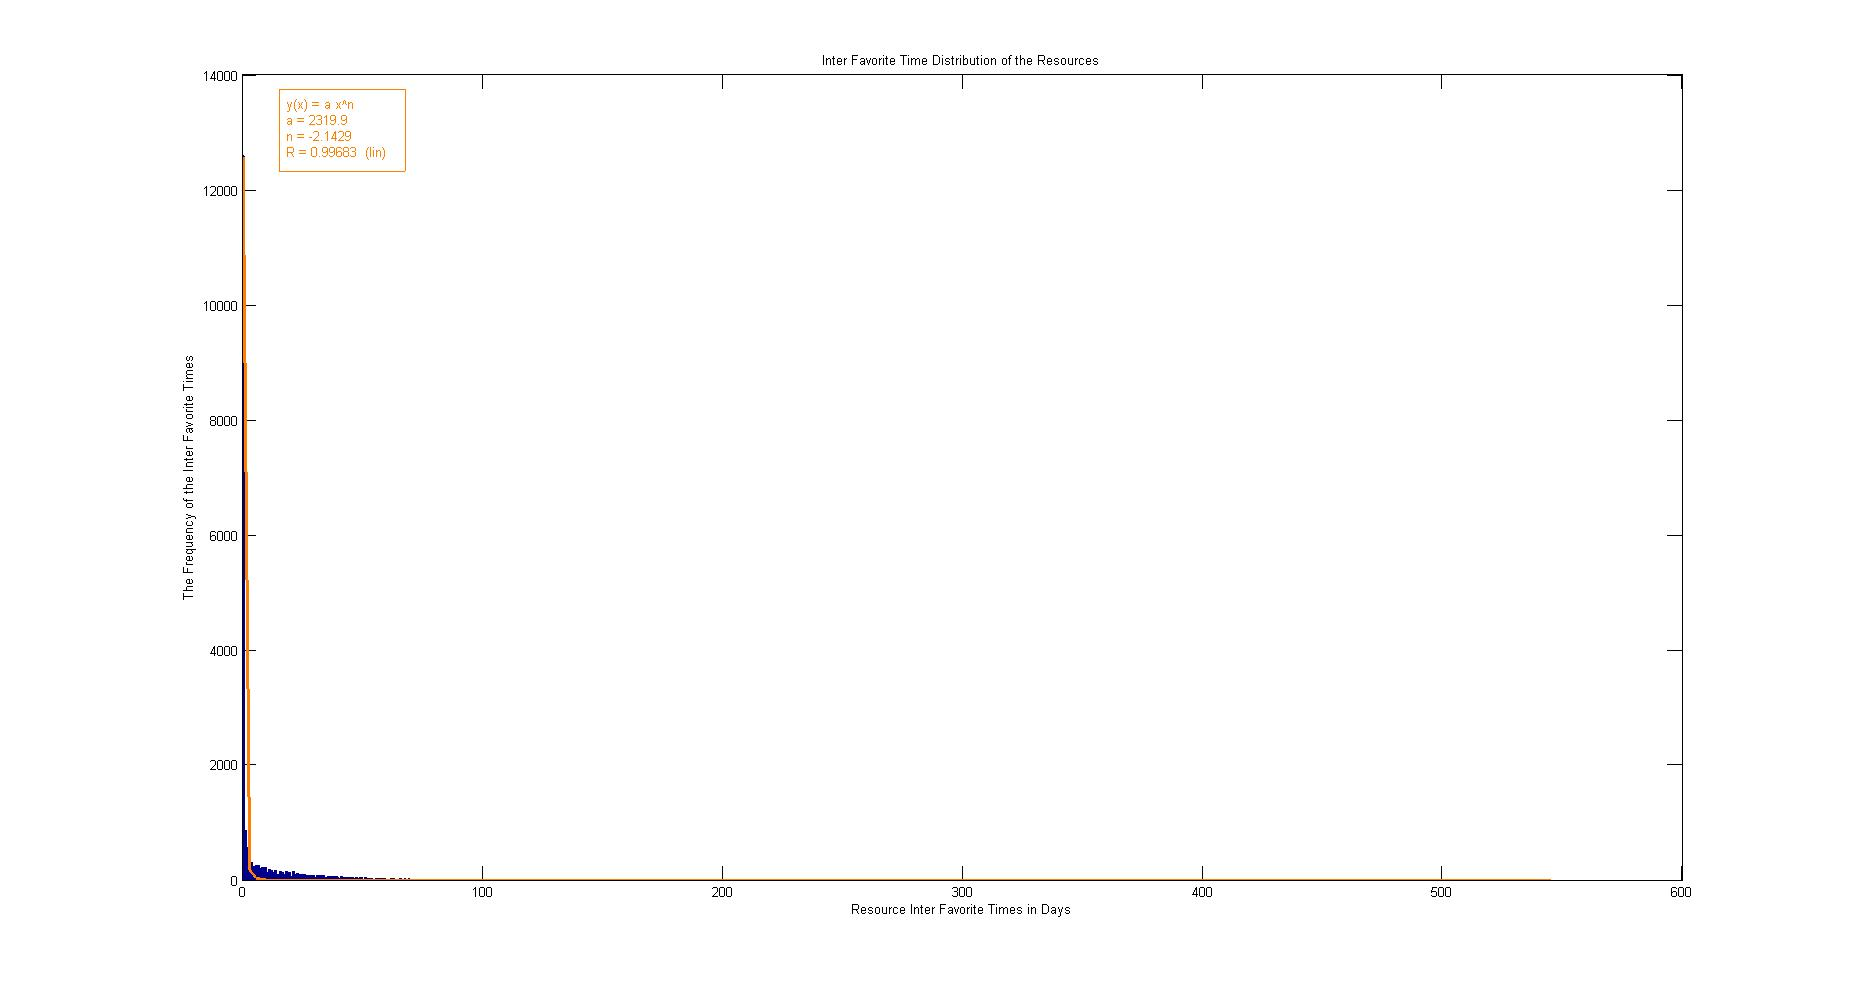
\includegraphics[width=200mm]{resInterDist.jpg}
	\caption{Inter Favorite Time Distribution}	
	\end{figure}

	\clearpage

	\section{Average Statistics of the Power Laws}

	\subsection{User}

	\begin{center}
	\begin{tabular}{|p{5cm}|p{5cm}|}
	\hline
	Produce List Size & 0.79 resources\\
	\hline
	Favorite List Size & 2.0241 resource\\
	\hline
	Inter Favorite Time & 12.85 days\\
	\hline
	\end{tabular}
	\end{center}

	\subsection{Resource}

	\begin{center}
	\begin{tabular}{|p{5cm}|p{5cm}|}
	\hline
	Favorite List Size & 2.55 users\\
	\hline
	Inter Favorite Time & 14.72 days\\
	\hline
	\end{tabular}
	\end{center}	

	\section{Classification}

	\par \hspace{0.6cm} Initially, we normalized cumulative favorite list of the users and resources with respect to their life time. As a result, we realized that there can be three type distribution. Class 1 is the above of the $y = x$ line. Class 2 is nearly $y = x$ line and finally Class 3 is the below of the line.  \\

	\large{Steps of Classification:}
	\normalsize
	\begin{itemize}
	\item Normalize Favorite List Size
	\item Normalize Life Time
	\item Calculate correlation with $y = x$ with 95%
	\item If correlates, set it to Class 2
	\item Else calculate average difference from $ y = x $
	\item If difference is positive, it is Class 1 else Class 3
	\end{itemize}

	\vspace{-5cm}
	\begin{figure}
	\hspace{-3.7cm}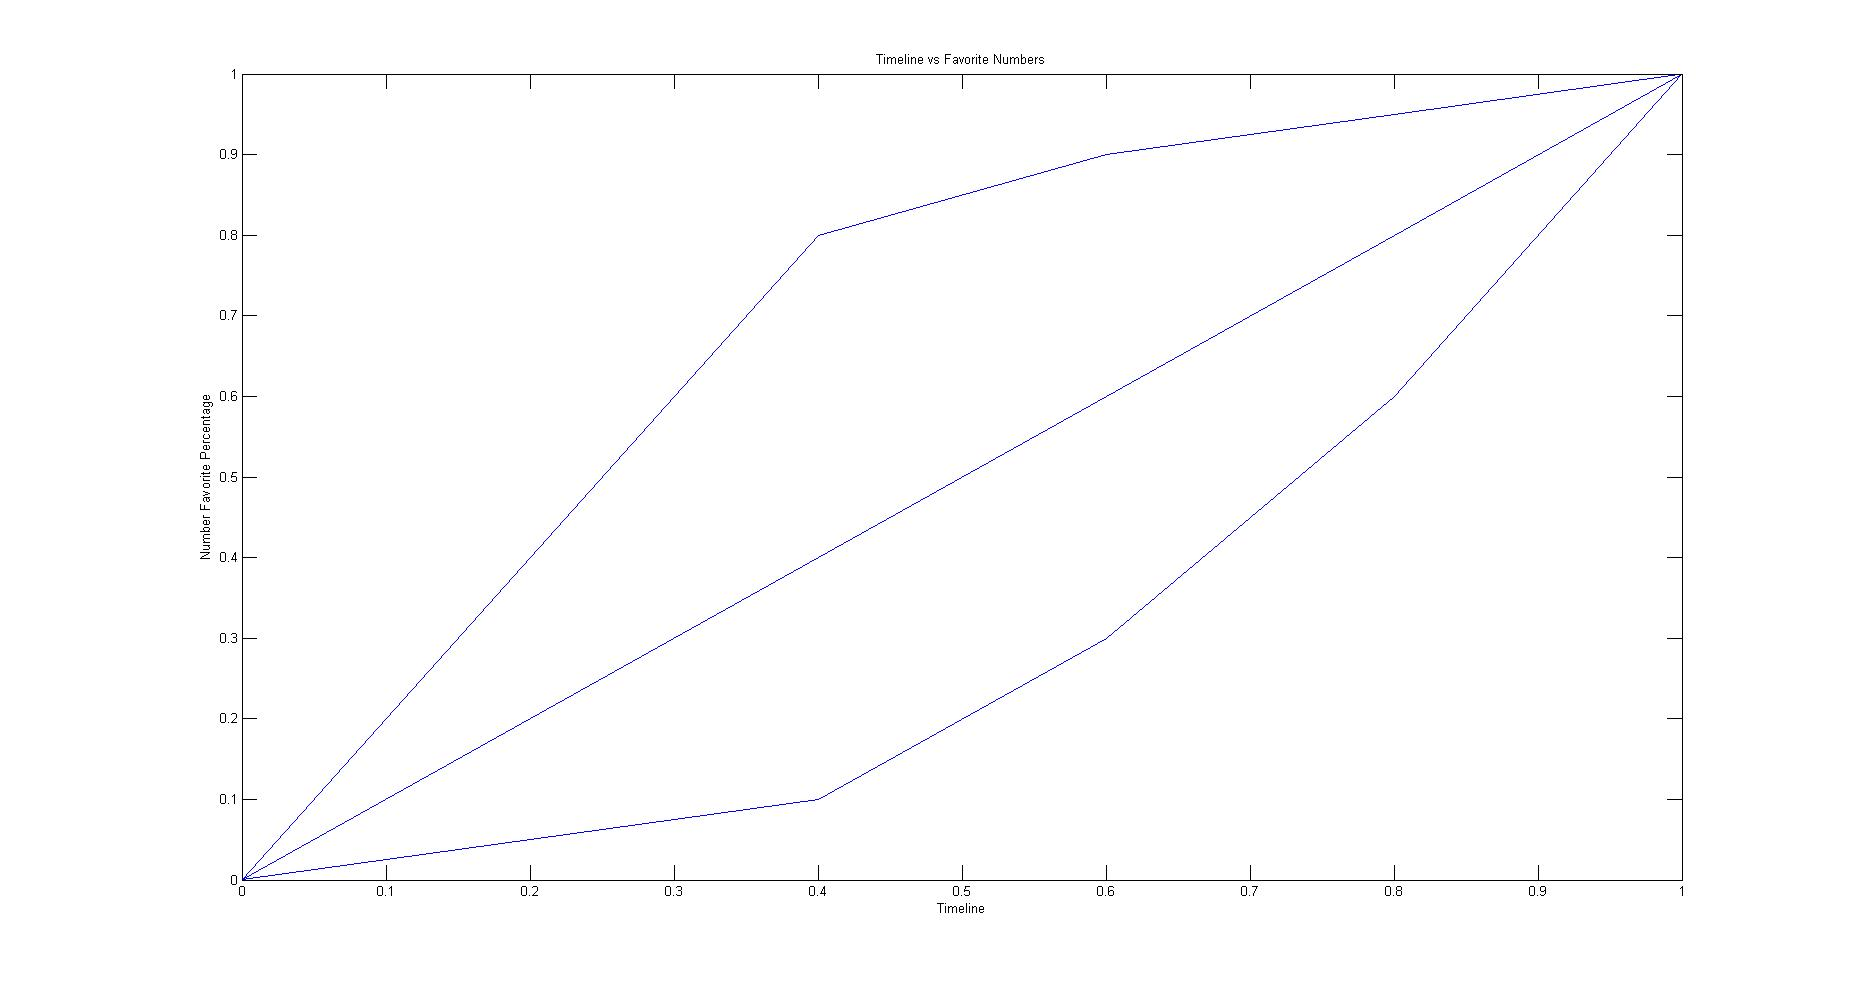
\includegraphics[width=200mm]{timelineFav.jpg}
	\caption{Class Types}
	\end{figure}

	\clearpage

	\subsection{User}

	\begin{center}
	\textup{\Large User Classes}
	\begin{tabular}{|p{6.5cm}|p{6.5cm}|}
	\hline
	Class 1 &  30509 \\ 
	\hline
	Class 2 & 7501 \\
	\hline
	Class 3 & 467\\
	\hline
	\end{tabular}
	\end{center}

	\subsection{Resource}

	\begin{center}
	\textup{\Large Resource Classes}
	\begin{tabular}{|p{6.5cm}|p{6.5cm}|}
	\hline
	Class 1 &  16109 \\ 
	\hline
	Class 2 & 6634 \\
	\hline
	Class 3 & 66 \\
	\hline
	\end{tabular}
	\end{center}

	\subsection{Implication of Classes}

	\par \hspace{0.6cm} For one artist to be influential, he must be a regular user of the DeviantART so this user must be in class 2 and one of 7501 artists.

	Class 1 resources are just fashion because they are popular for just a small time frame.  Class 2  resources has intrinsically  a good quality, actually their emergency values are high and they don't need any external factors to be popular. However, Class 3 resources do a jump in their timeline by an effect of the external factor. Since we assume this external factor to be a favorite relation, we can easily see the most influential user in the timeline of these users. Moreover, we must look 12-13-14 days prior to jump because users have add new favorites in 12 days at average and resources have been added as favorite in 14 days at average. \\

	\subsection{Differences in the timeline of resources}

	\par \hspace{0.6cm} We normalized favorite list size and timeline of the resources. Then, we calculated the difference from $y = x$ line. The more negative value is, the more resources are class 1 type of. \\

	\vspace{-5cm}
	\begin{figure}
	\hspace{-3.7cm}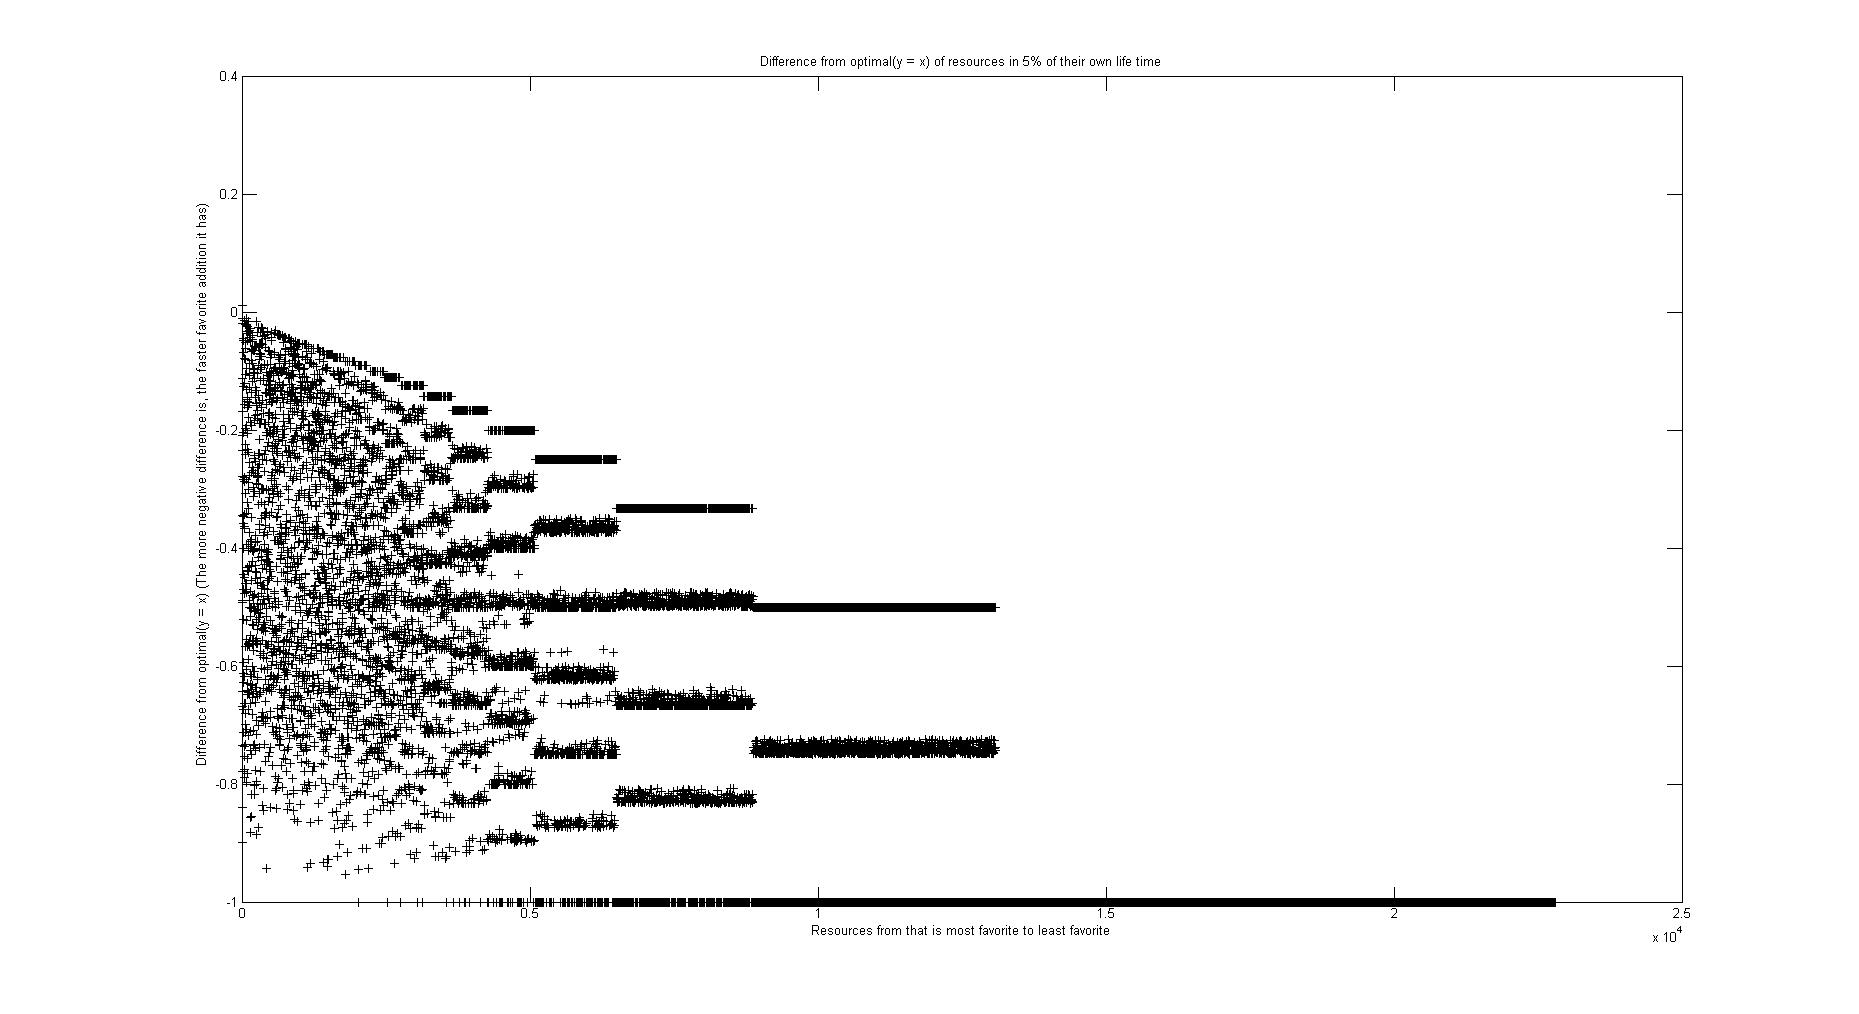
\includegraphics[width=200mm]{first.jpg}
	\caption{Difference Scatter Plot in 5\% Lifetime}
	\end{figure}

	\vspace{-5cm}
	\begin{figure}
	\hspace{-3.7cm}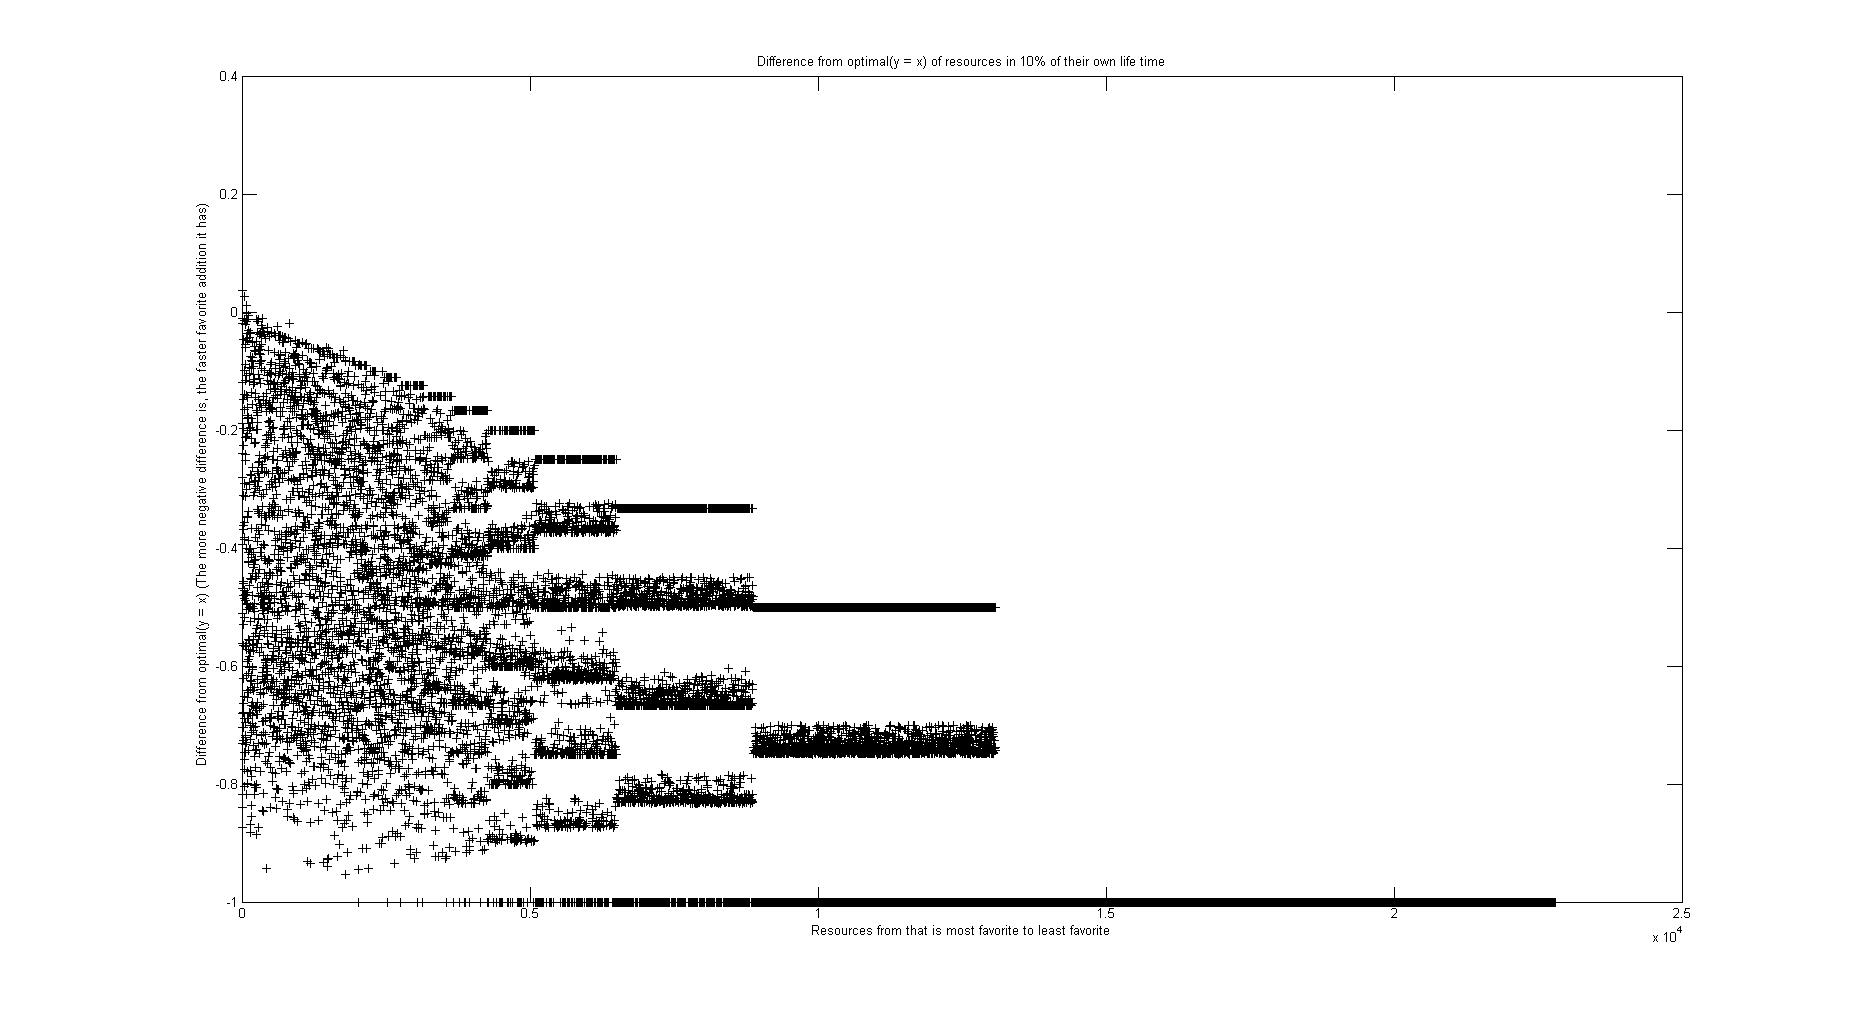
\includegraphics[width=200mm]{second.jpg}
	\caption{Difference Scatter Plot in 10\% Lifetime}
	\end{figure}

	\vspace{-5cm}
	\begin{figure}
	\hspace{-3.7cm}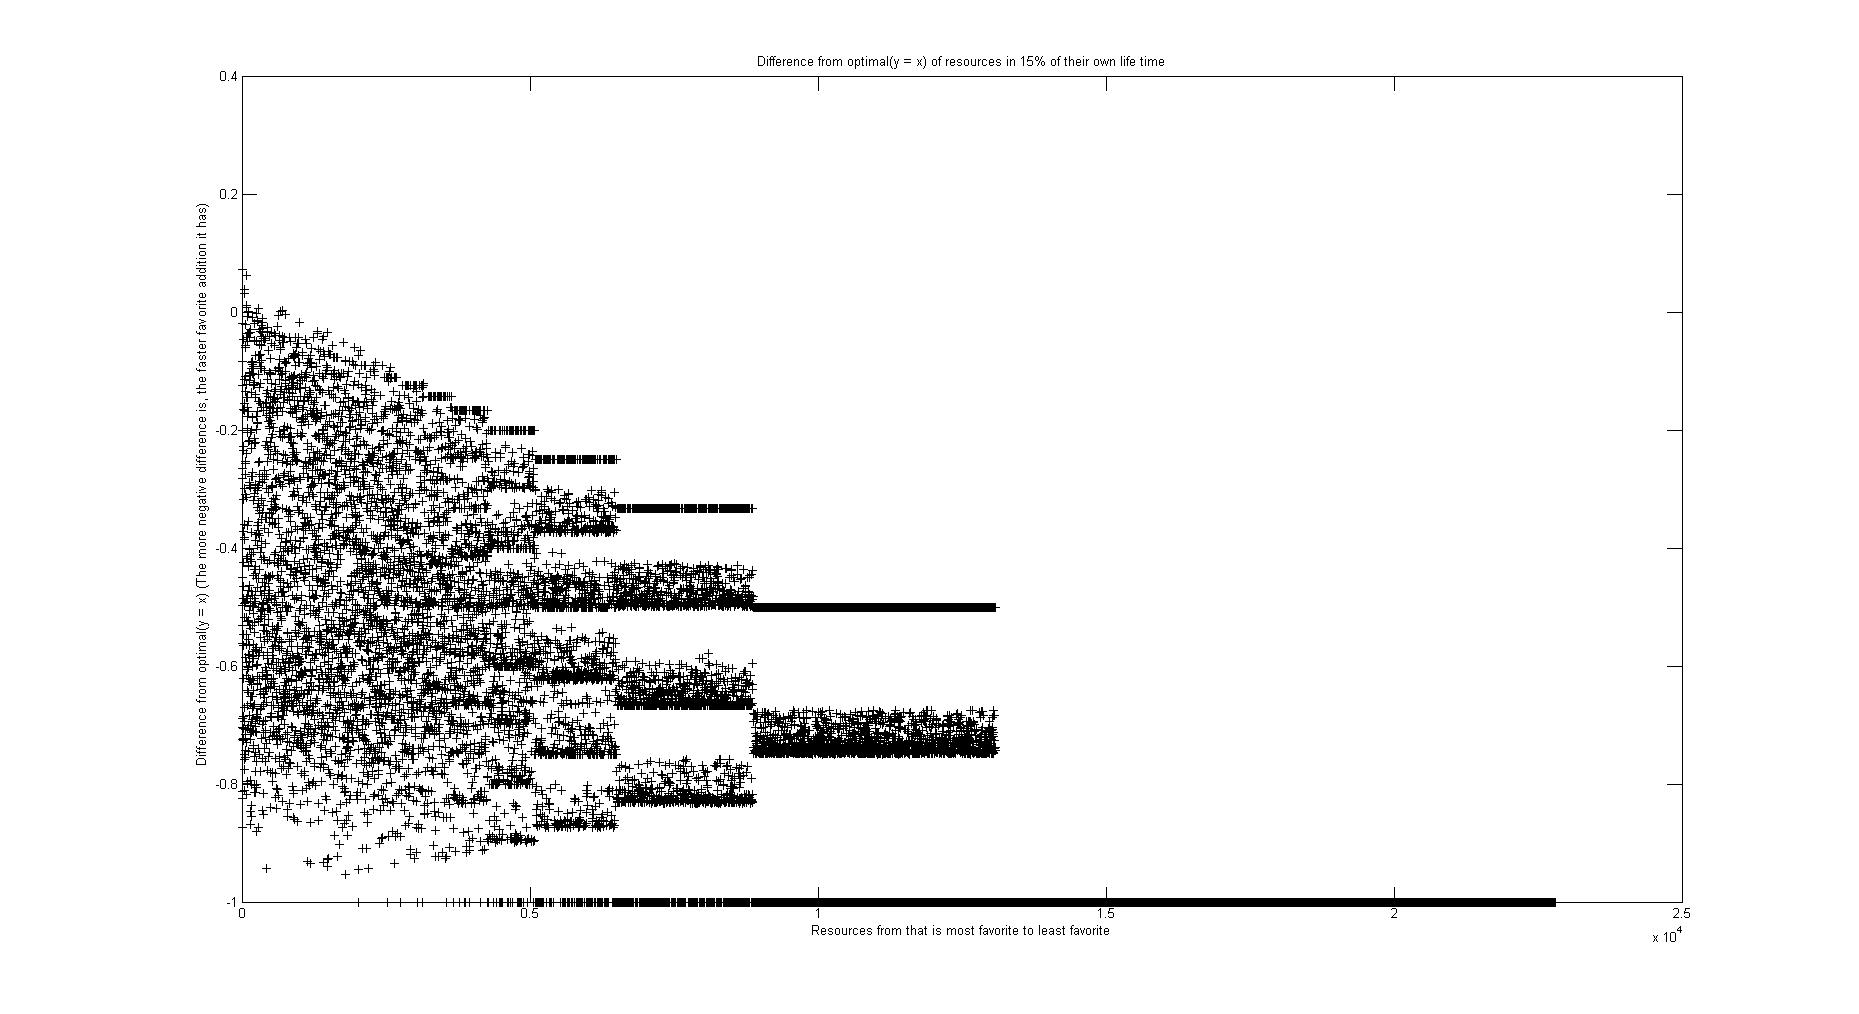
\includegraphics[width=200mm]{third.jpg}
	\caption{Difference Scatter Plot in 15\% Lifetime}
	\end{figure}

	\vspace{-5cm}
	\begin{figure}
	\hspace{-3.7cm}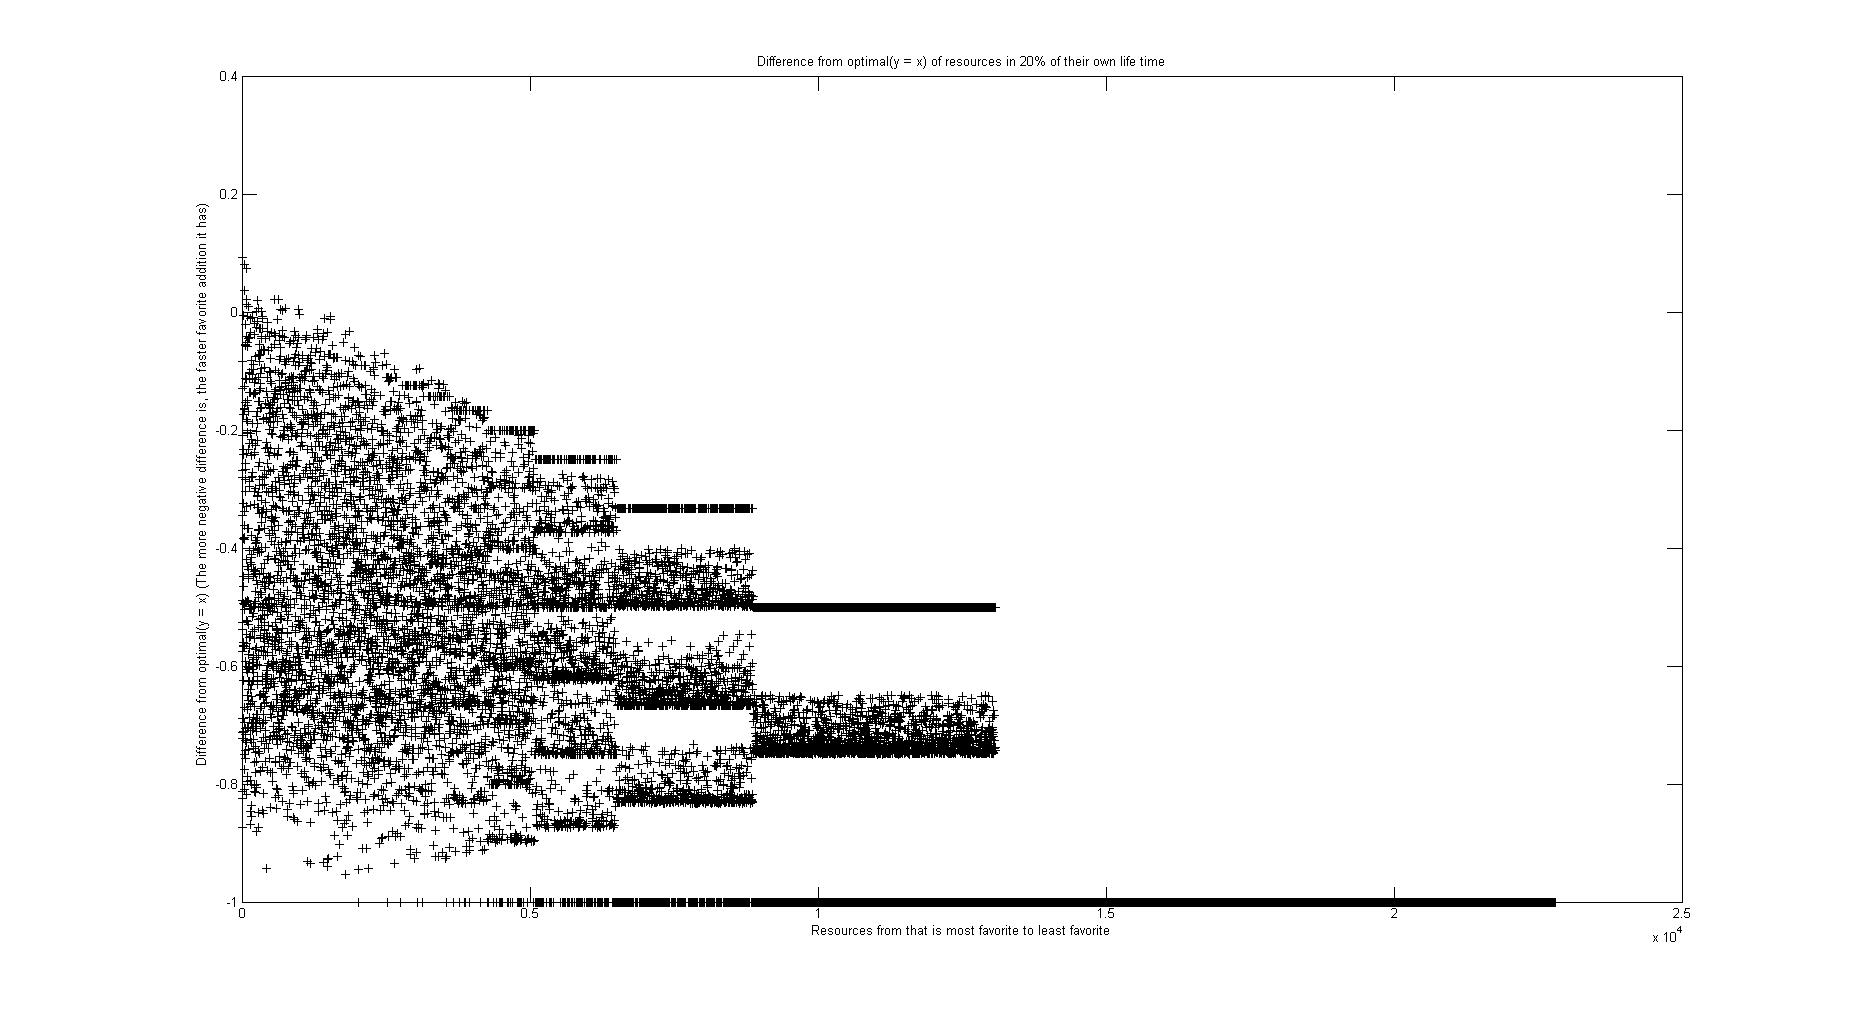
\includegraphics[width=200mm]{fourth.jpg}
	\caption{Difference Scatter Plot in 20\% Lifetime}
	\end{figure}

	\vspace{-5cm}
	\begin{figure}
	\hspace{-3.7cm}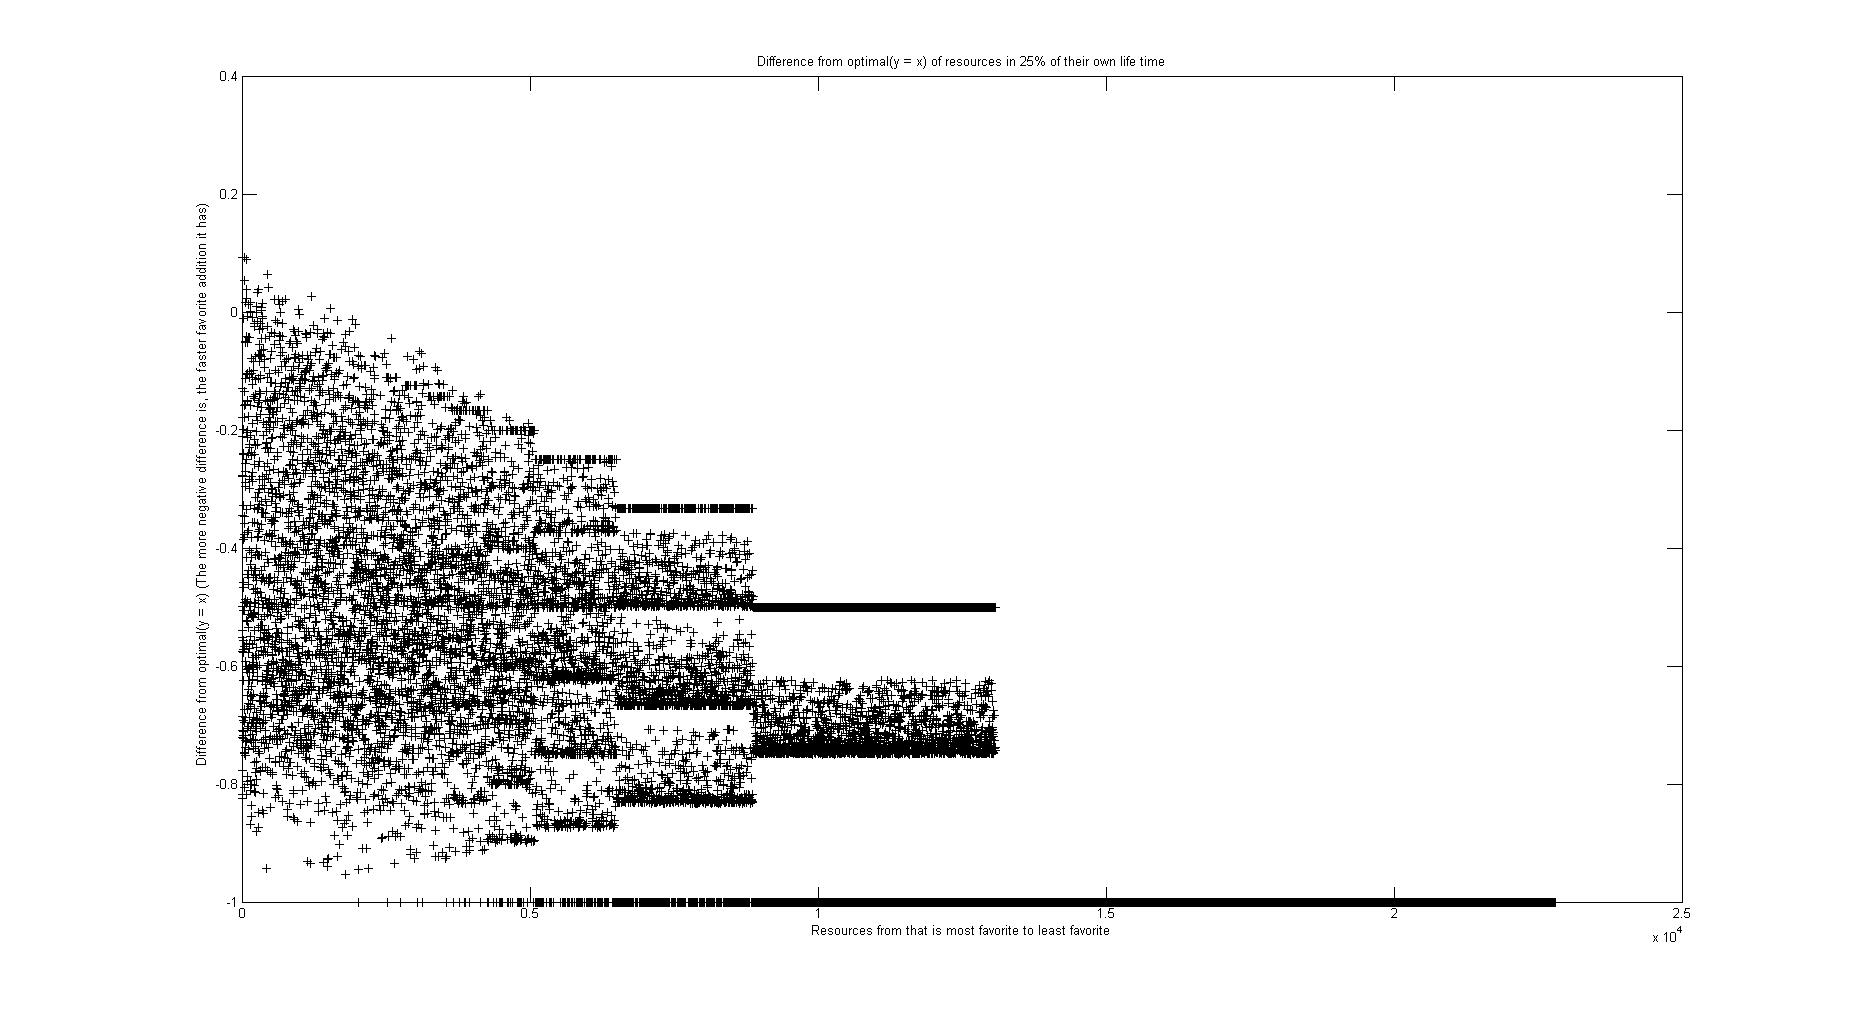
\includegraphics[width=200mm]{fifth.jpg}
	\caption{Difference Scatter Plot in 25\% Lifetime}
	\end{figure}

	\vspace{-5cm}
	\begin{figure}
	\hspace{-3.7cm}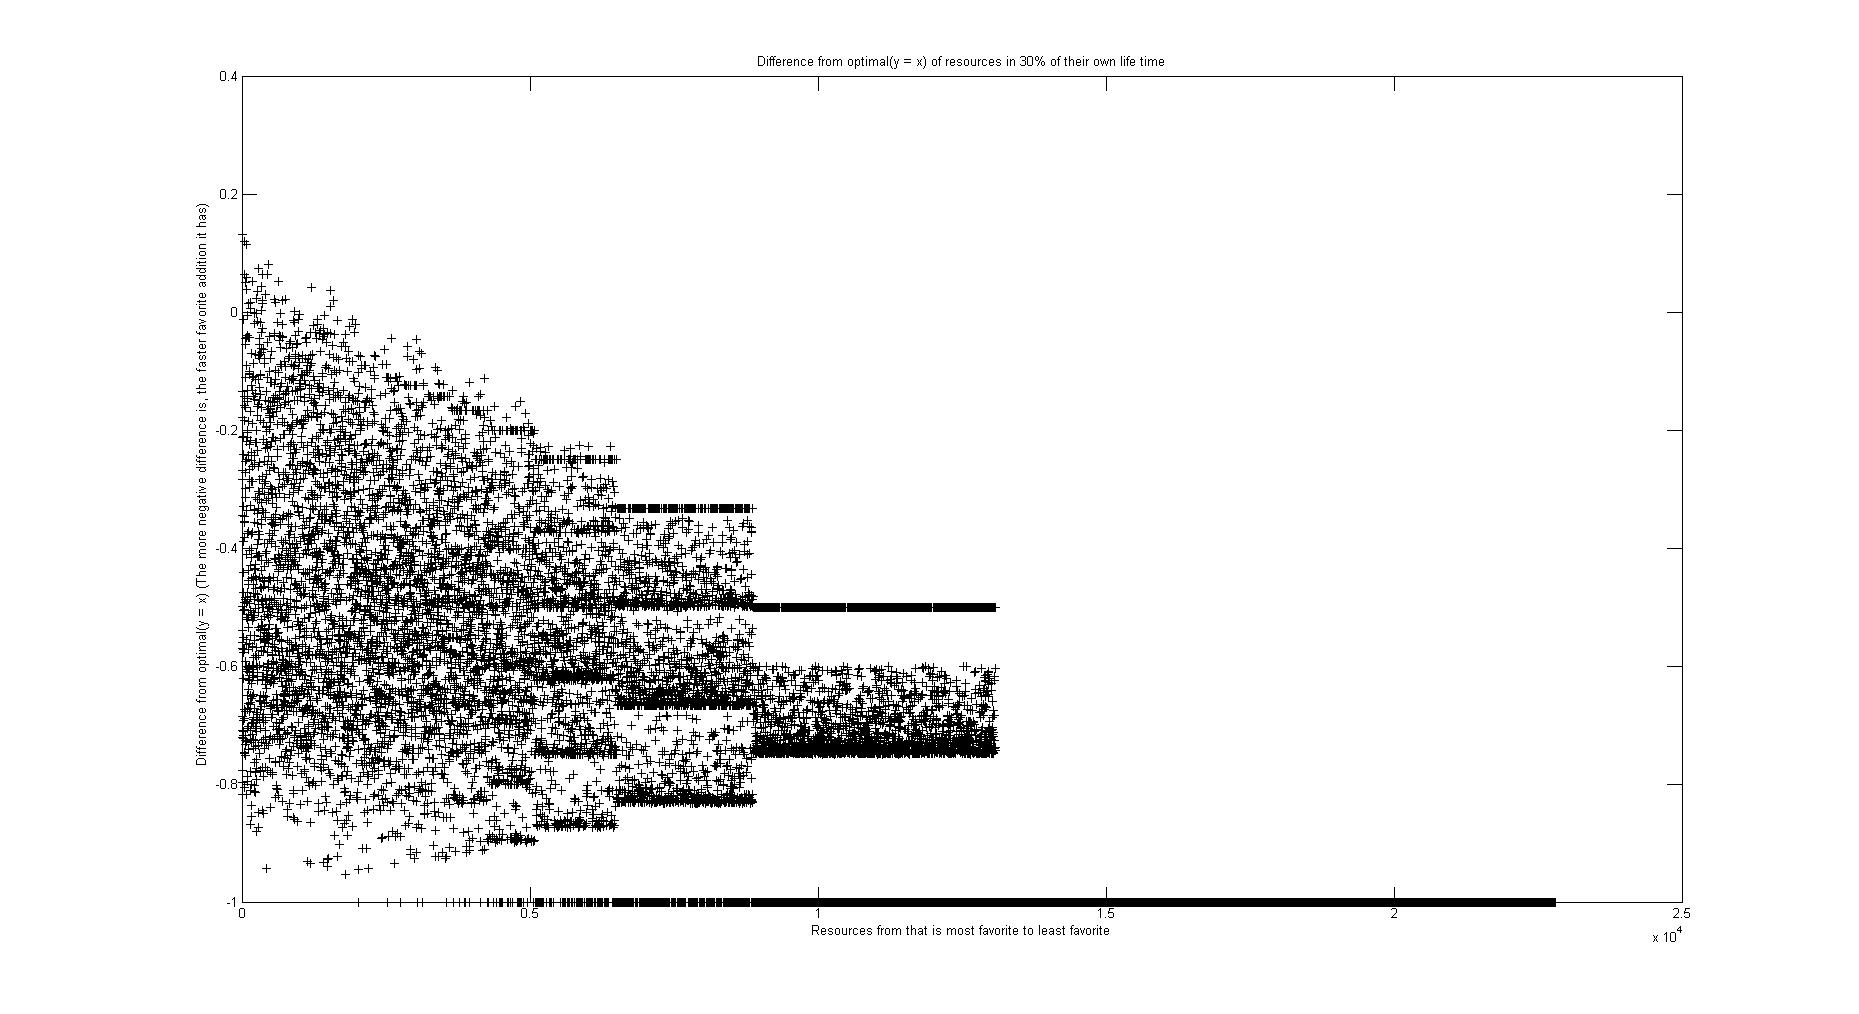
\includegraphics[width=200mm]{sixth.jpg}
	\caption{Difference Scatter Plot in 30\% Lifetime}
	\end{figure}

	\vspace{-5cm}
	\begin{figure}
	\hspace{-3.7cm}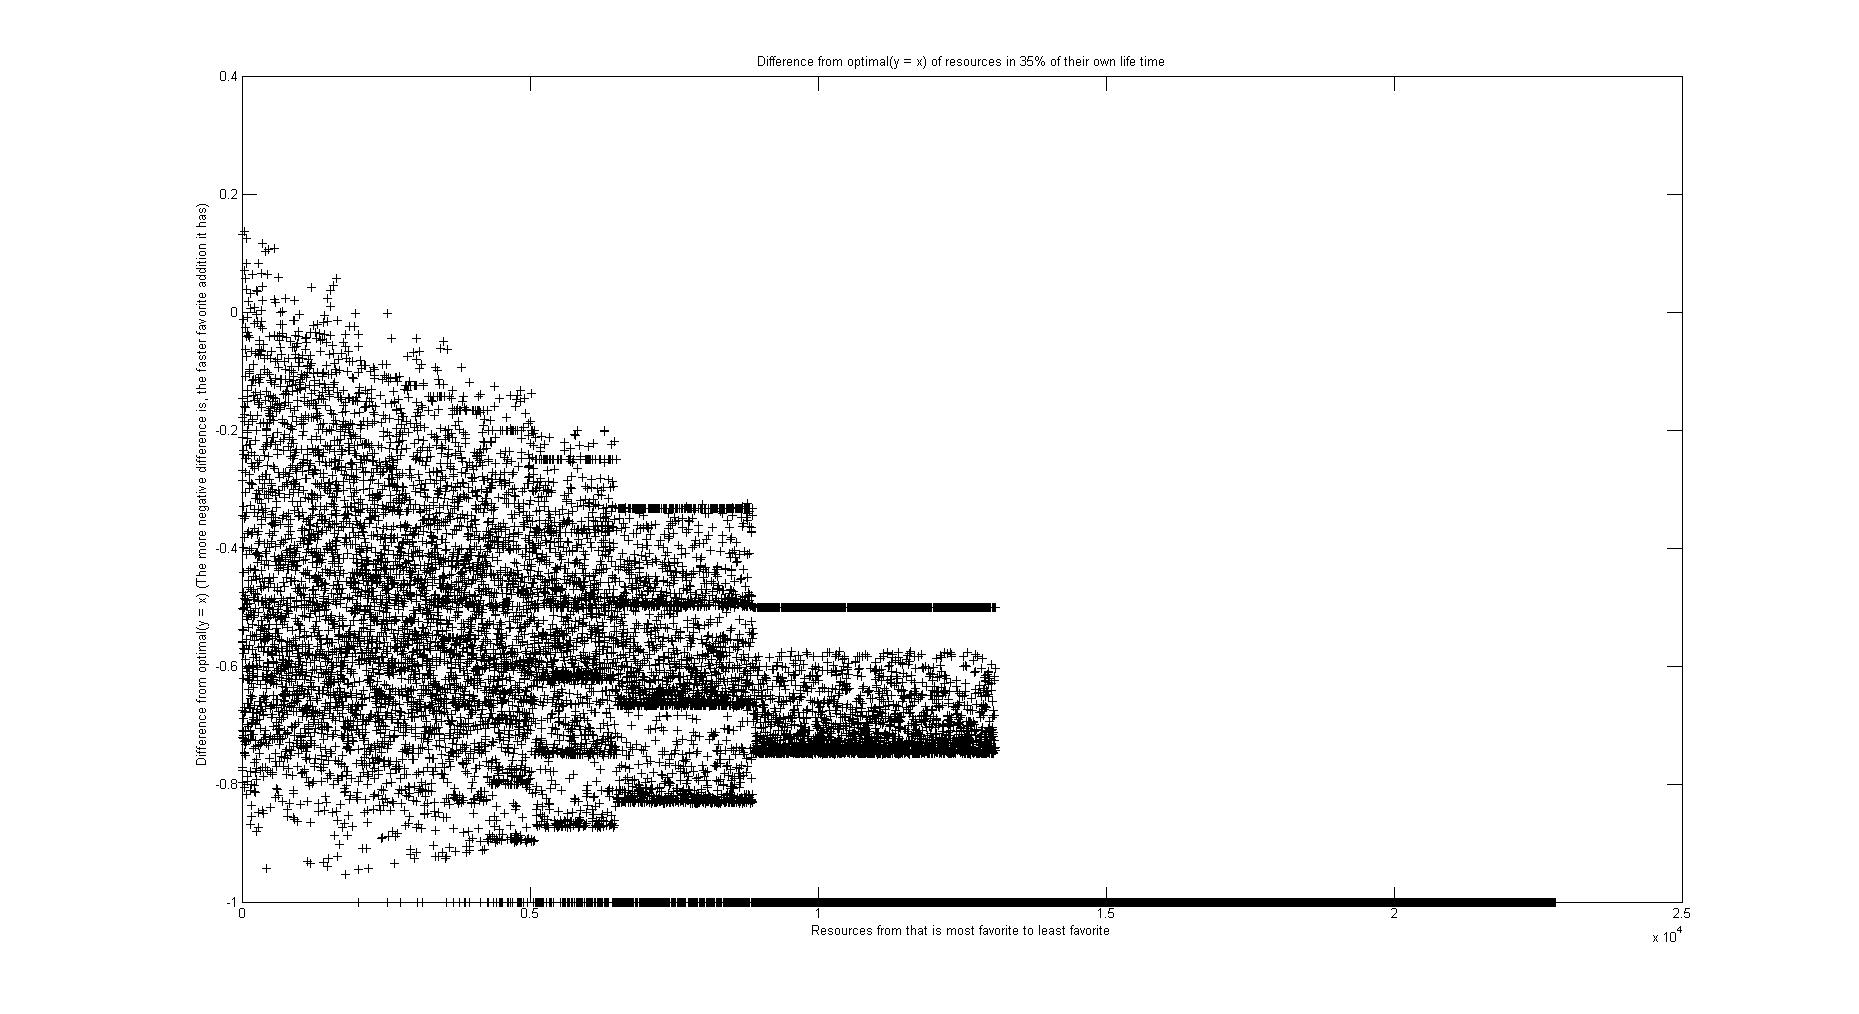
\includegraphics[width=200mm]{seventh.jpg}
	\caption{Difference Scatter Plot in 35\% Lifetime}
	\end{figure}

	\vspace{-5cm}
	\begin{figure}
	\hspace{-3.7cm}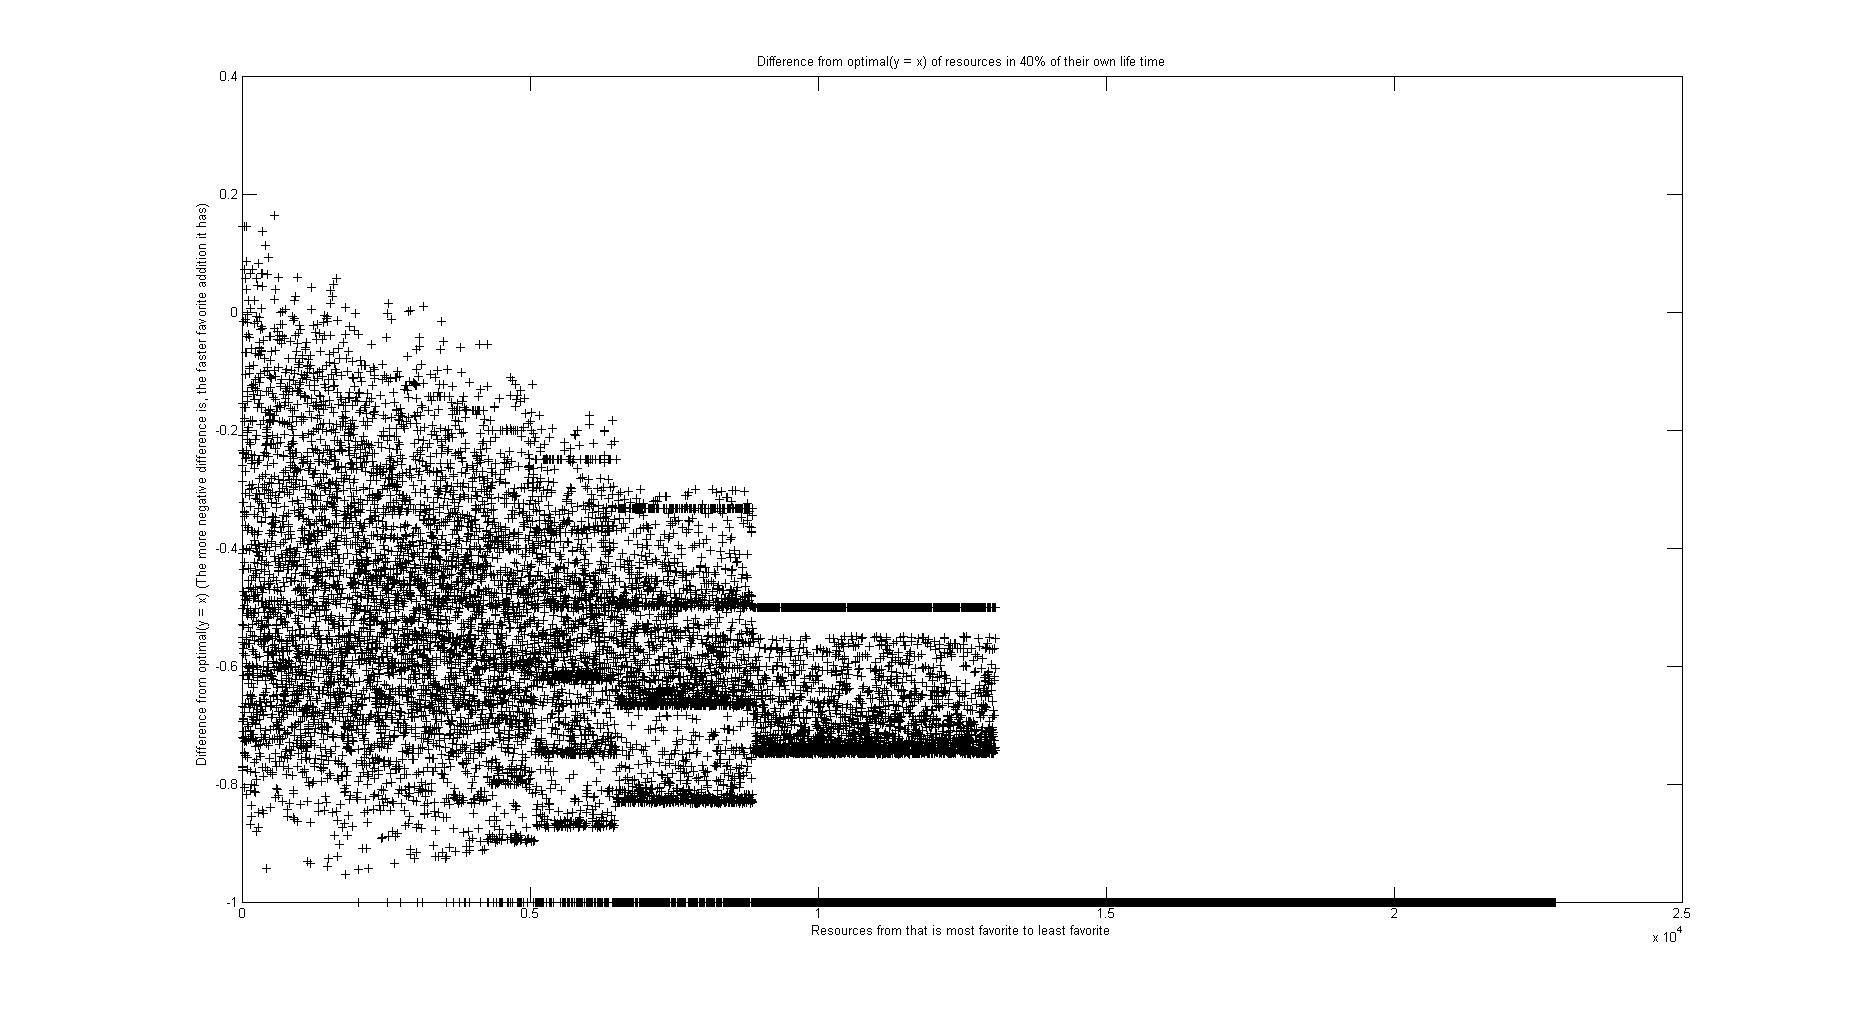
\includegraphics[width=200mm]{eighth.jpg}
	\caption{Difference Scatter Plot in 40\% Lifetime}
	\end{figure}

	\vspace{-5cm}
	\begin{figure}
	\hspace{-3.7cm}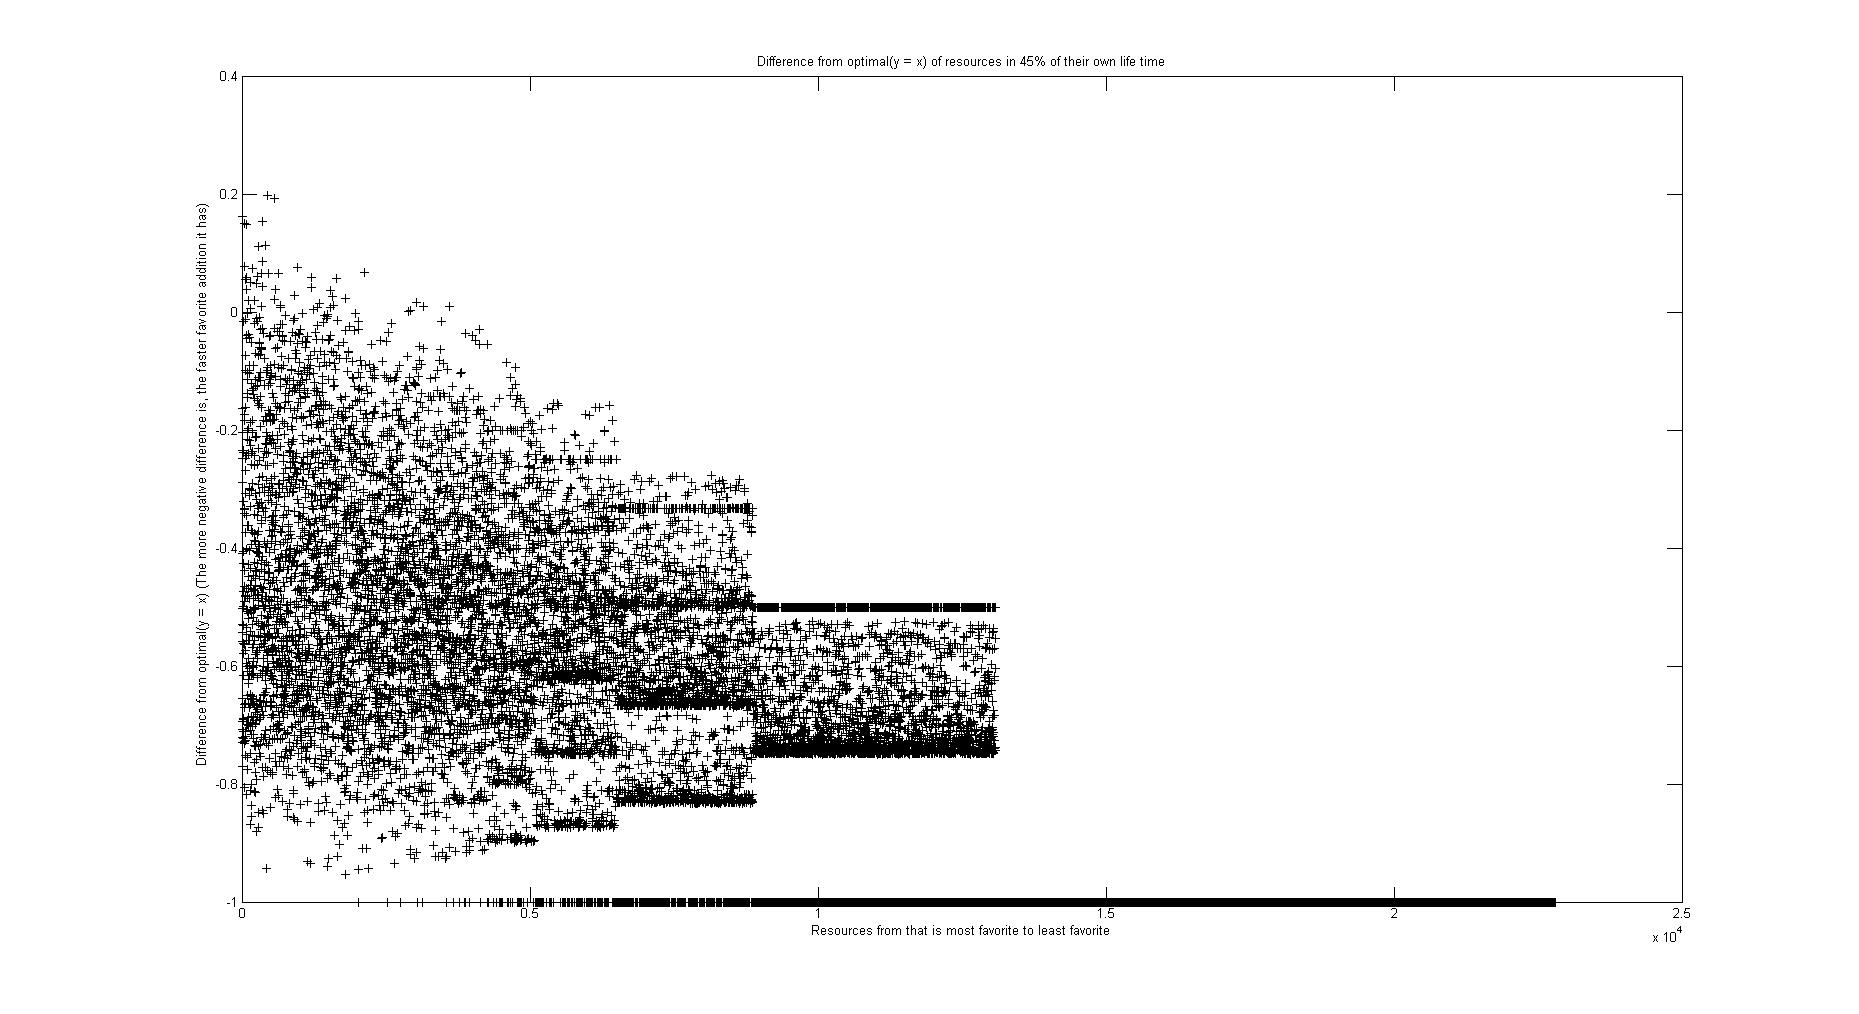
\includegraphics[width=200mm]{nineth.jpg}
	\caption{Difference Scatter Plot in 45\% Lifetime}
	\end{figure}
	
	\vspace{-5cm}
	\begin{figure}
	\hspace{-3.7cm}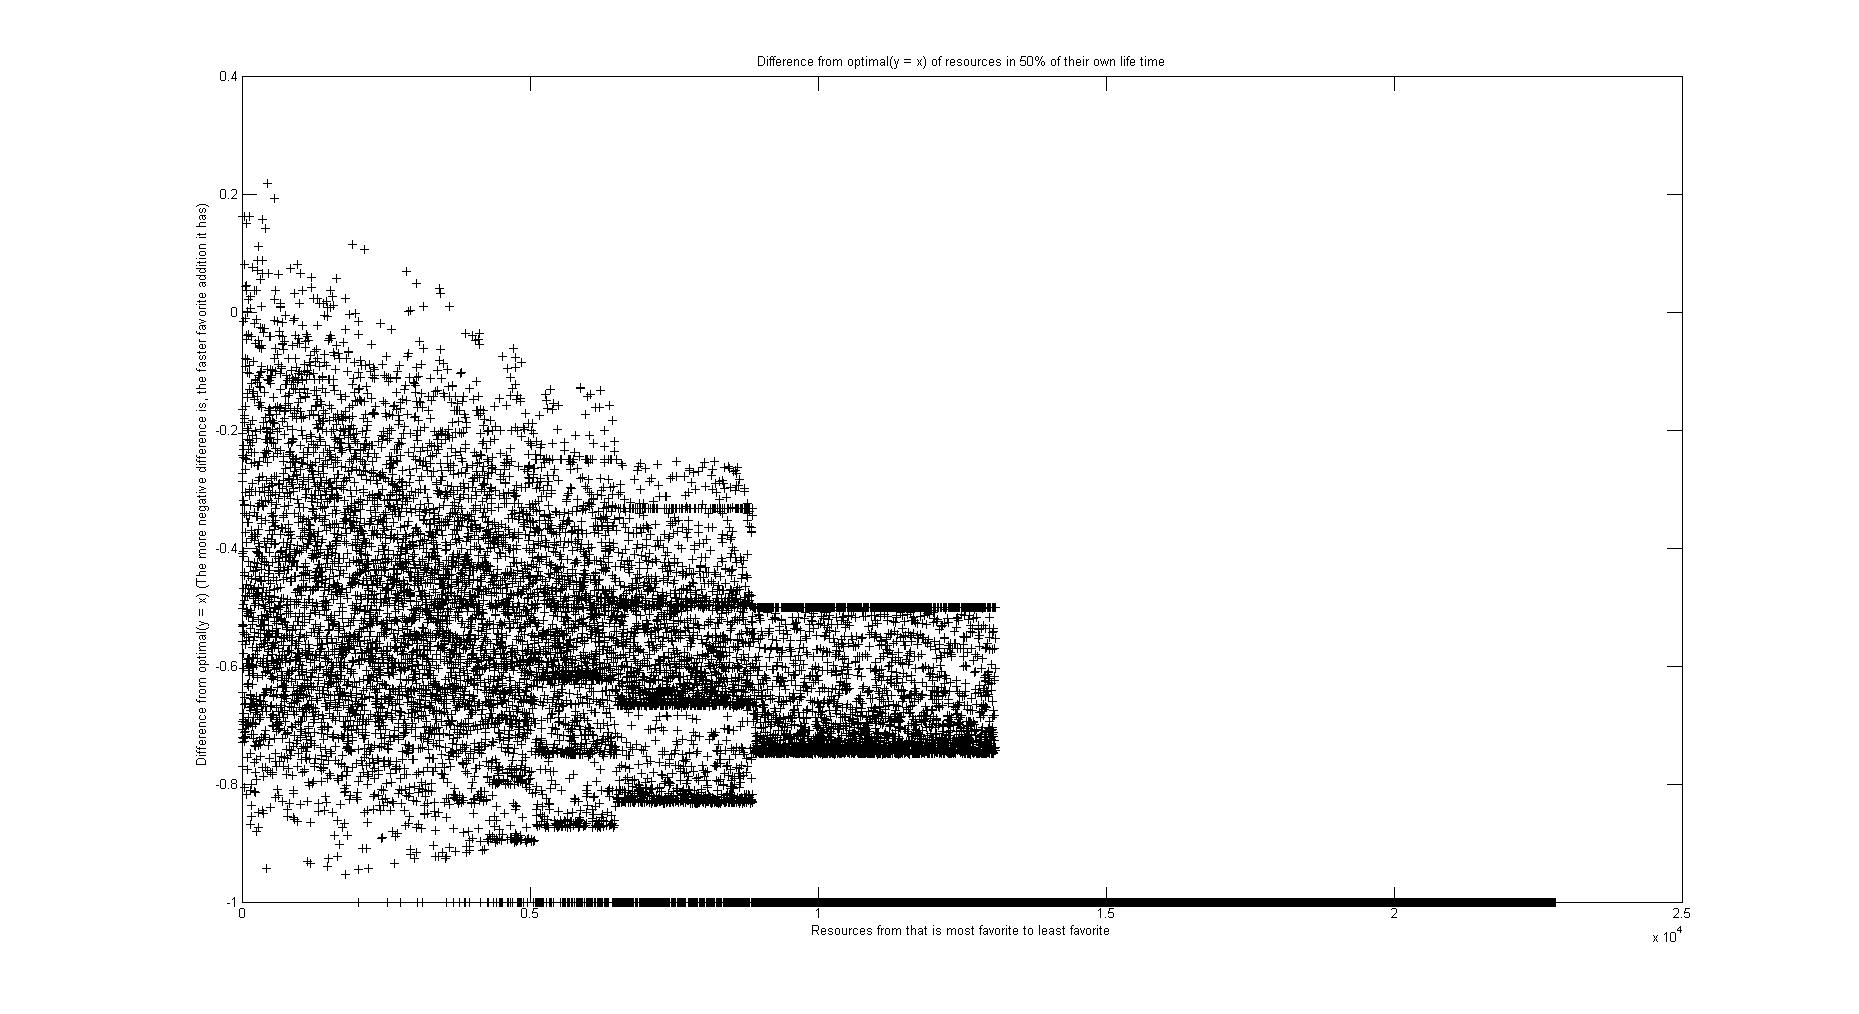
\includegraphics[width=200mm]{tenth.jpg}
	\caption{Difference Scatter Plot in 50\% Lifetime}
	\end{figure}

	\vspace{-5cm}
	\begin{figure}
	\hspace{-3.7cm}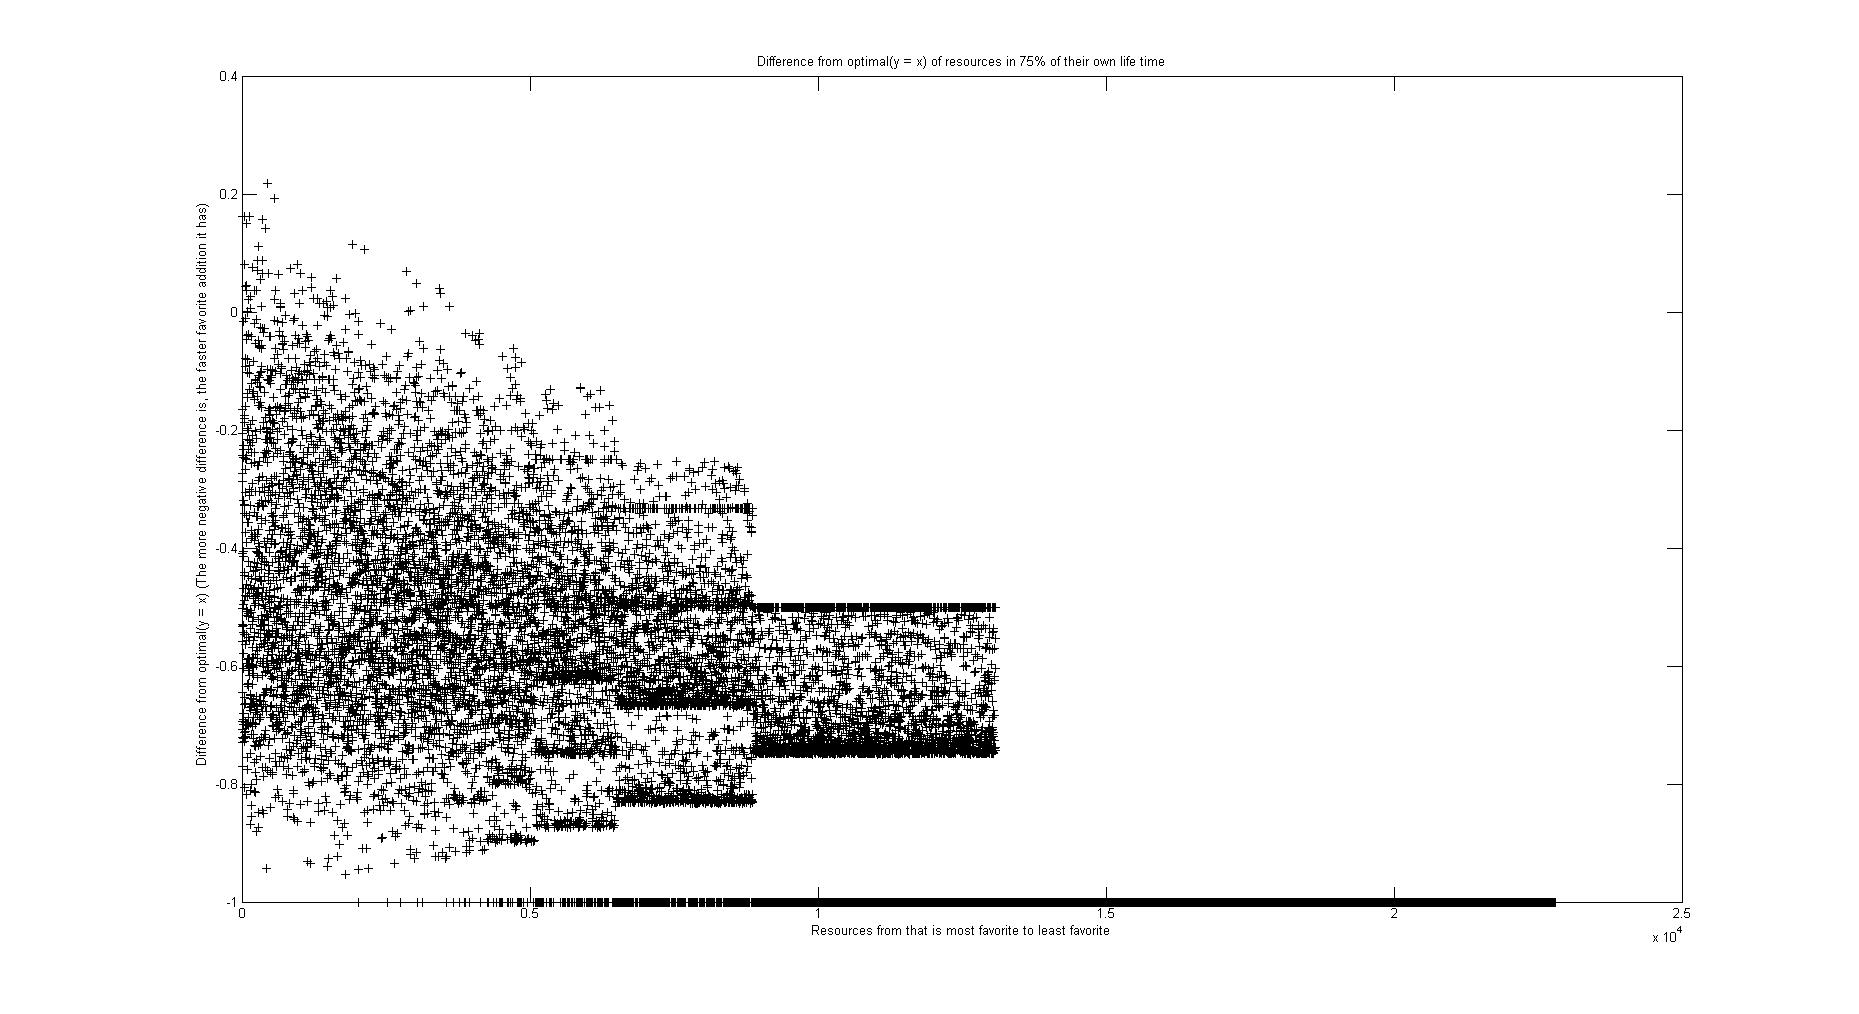
\includegraphics[width=200mm]{seventyfive.jpg}
	\caption{Difference Scatter Plot in 75\% Lifetime}
	\end{figure}
	
	\vspace{-5cm}
	\begin{figure}
	\hspace{-3.7cm}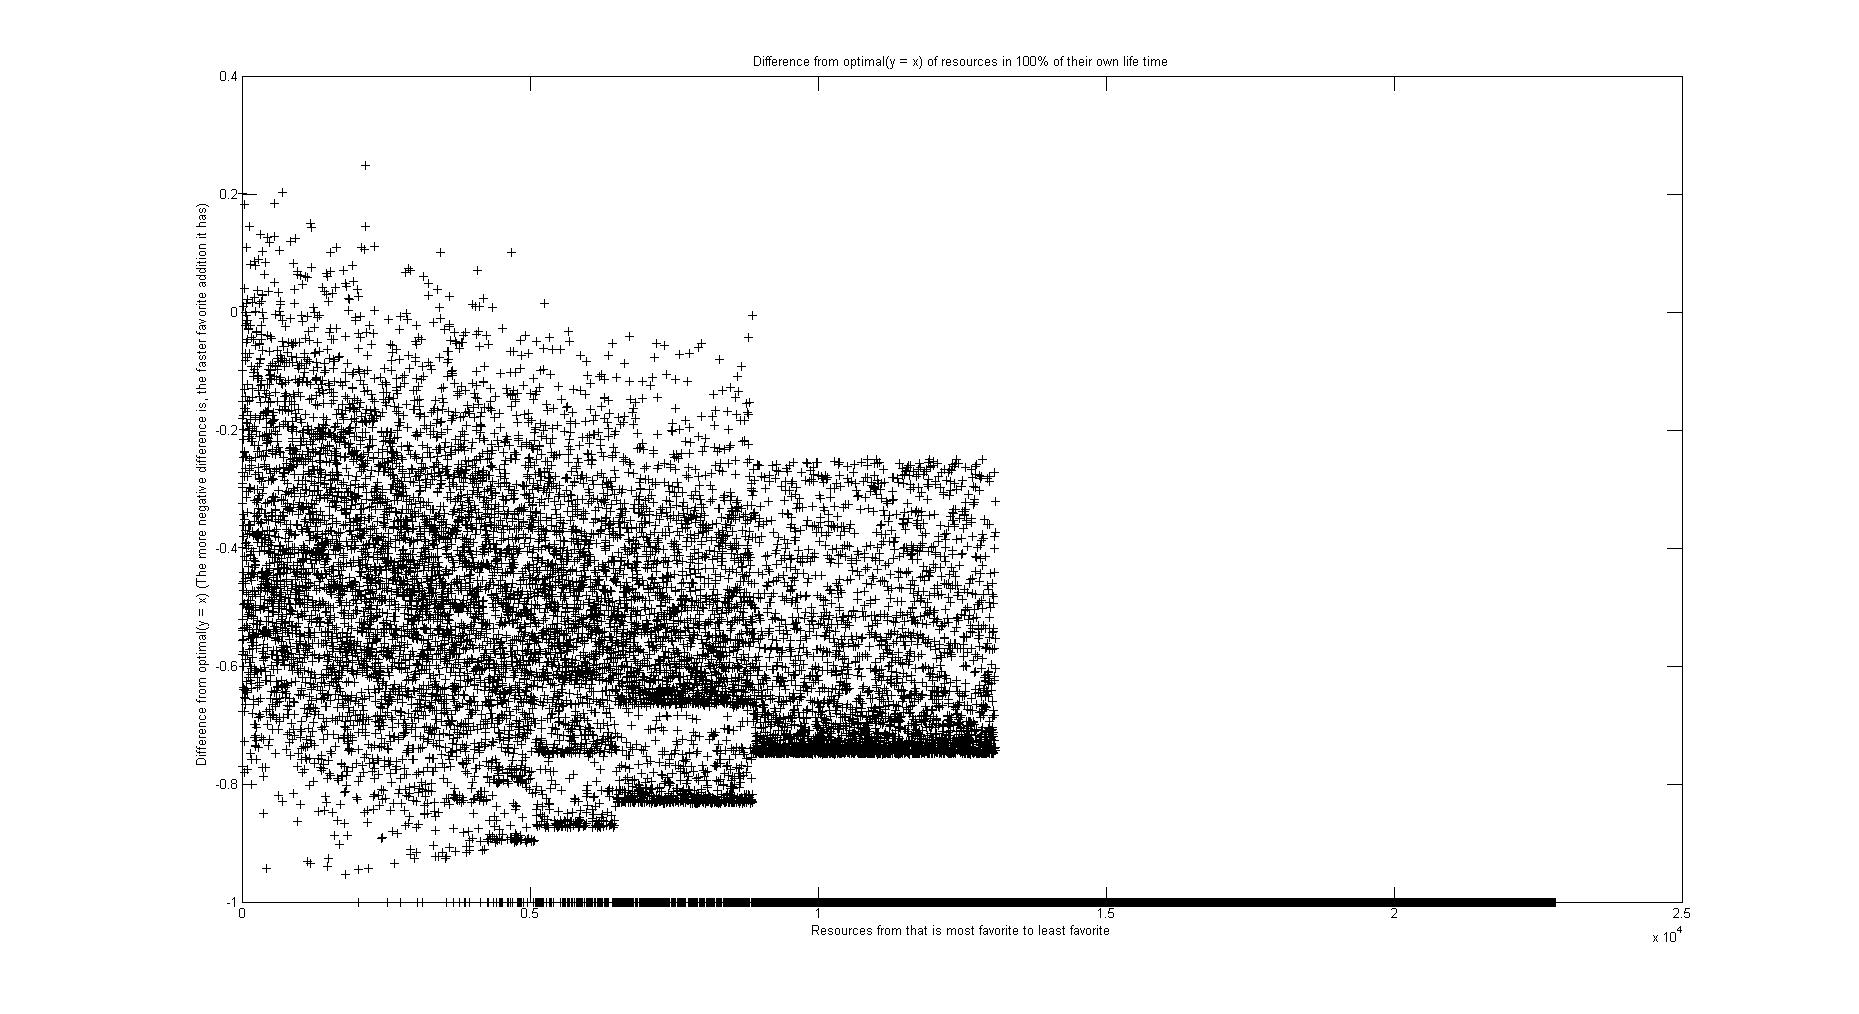
\includegraphics[width=200mm]{hundred.jpg}
	\caption{Difference Scatter Plot in 100\% Lifetime}
	\end{figure}

	\vspace{-5cm}
	\begin{figure}
	\hspace{-3.7cm}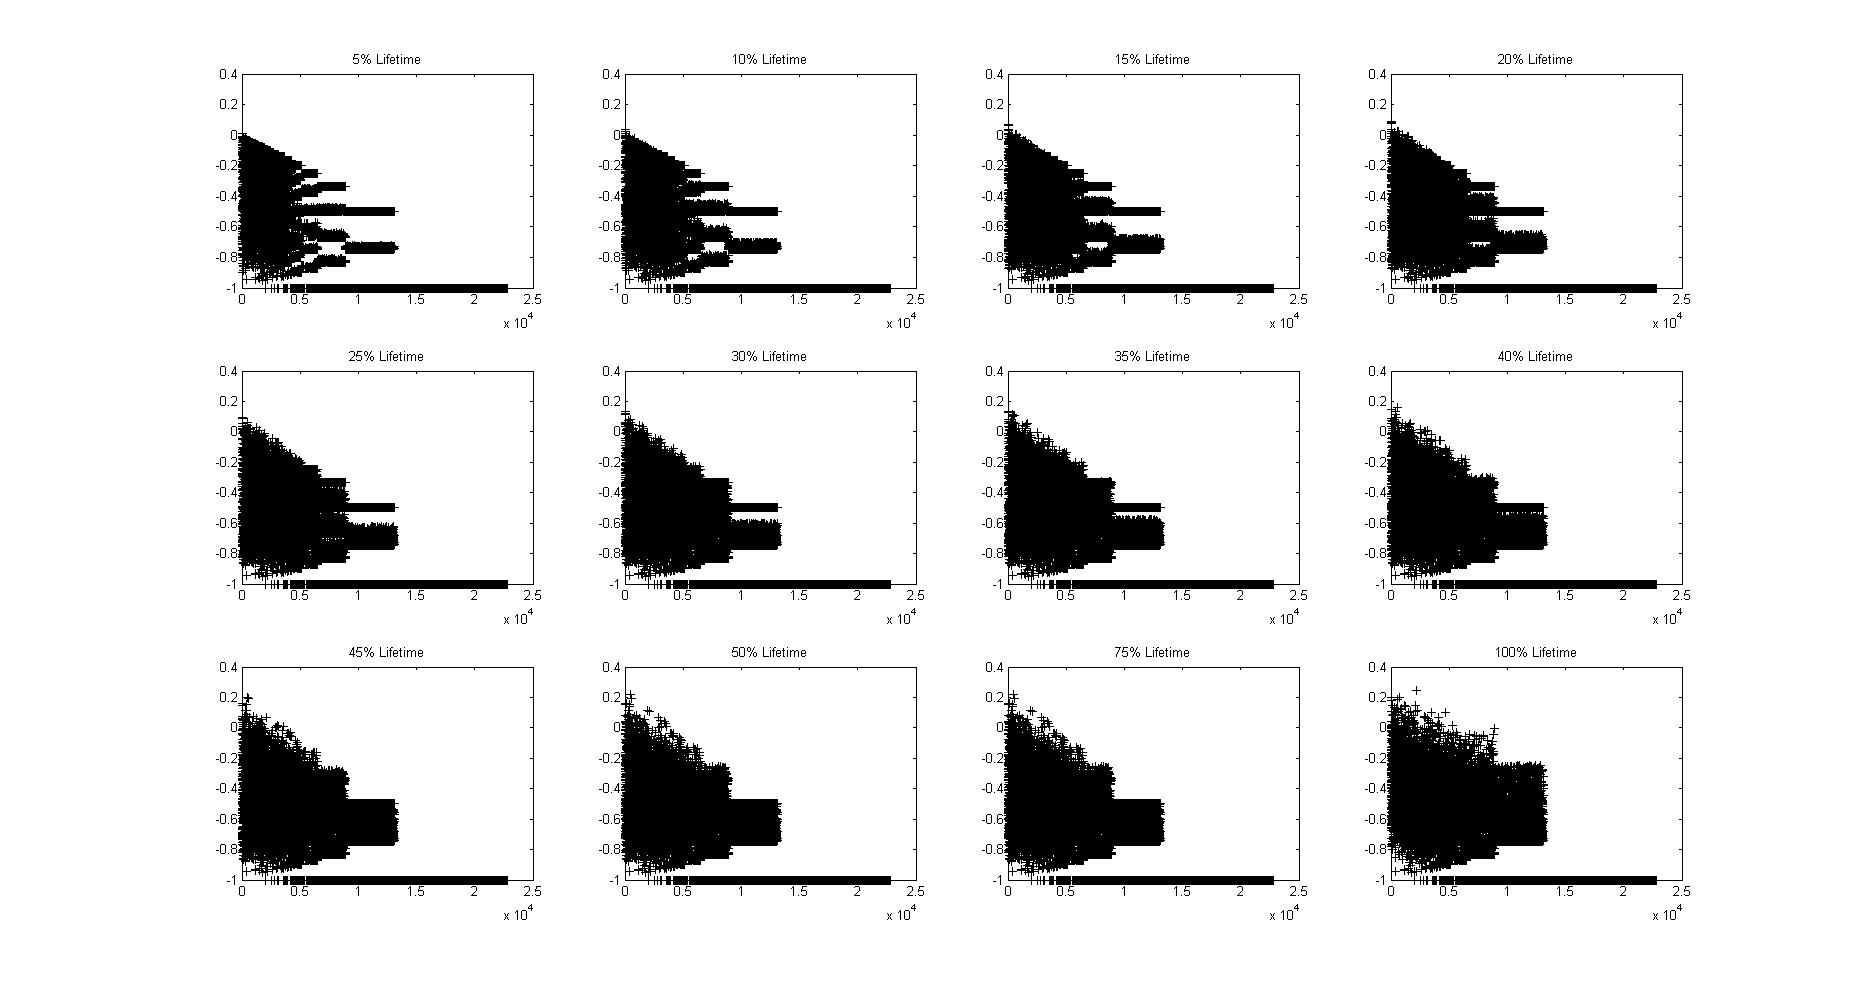
\includegraphics[width=200mm]{total.jpg}
	\caption{Difference Scatter Plot all in one}
	\end{figure}

\chapter{Conclusions and Future Work}

	\begin{itemize}
	\item We suggested an algorithm  to find the most influential user in the social networks. Then, we analyzed deviantArt network and found that parameters of the network coincides with algorithm parameters.

	\item The most important factor for algorithm is the user authority distribution.
	\item Resource distribution can interfere with authority values.
	\item These findings are valid for whole network but we can mitigate them with above classification.
	\item The most influential user must use the site regularly because he can influence other users by only this way. Therefore, he must be in class 2.
	\item The effect of the most influential user can be seen on class 3 resources because these resources have small number favorites at the start but then there is a jump their favorite list size. If this jump is a result of influence of another user, we can find who he is  with  suggested algorithm but in the network there are a lot of info sources so the relative  effect of favorite relation should be analyzed further.
	\end{itemize}

\chapter{Appendix}

\begin{center}
\large
\textup{\textbf{Distributons of User and Resource Generation\\}}
\normalsize
\textup{These values are just runs of the distribution \emph{10,000} times}
\begin{tabular}{|c|c|c|}
\hline
\textbf{$n$} & \textbf{$\mu$} & \textbf{$\sigma^2$} \\
\hline
0 & 0.3327 & 0.0562\\
\hline
1 & 0.4178 & 0.0789 \\
\hline
2 & 0.3459 & 0.0694 \\
\hline
3 & 0.2791 & 0.0558 \\
\hline
4 & 0.2300 & 0.0425 \\
\hline
5 & 0.1903 & 0.0316 \\
\hline
6 & 0.1647 & 0.0267 \\
\hline
7 & 0.1415 & 0.0198 \\
\hline
8 & 0.1262 & 0.0158 \\
\hline
9 & 0.1097 & 0.0115 \\
\hline
10 & 0.1006 & 0.0102 \\
\hline
11 & 0.0903 & 0.0080 \\
\hline
12 & 0.0825 & 0.0069 \\
\hline
13 & 0.0765 & 0.0059 \\
\hline
14 & 0.0722 & 0.0052 \\
\hline
15 & 0.0663 & 0.0043 \\
\hline
16 & 0.0622 & 0.0039 \\
\hline
17 & 0.0581 & 0.0034 \\
\hline
18 & 0.0560 & 0.0032 \\
\hline
19 & 0.0520 & 0.0027 \\
\hline
20 & 0.0502 & 0.0025 \\
\hline
\end{tabular}
\end{center}

\clearpage

\chapter{References}

\begin{itemize}

\item \textbf{DeviantART} 

http://www.deviantart.com 

\item \textbf{DeviantART in Spotlight: A Network of Arts and Artists }

Almila Akdag Salah, Albert Ali Salah, Bart Buter, Nick Dijkshoorn, Davide Modolo, Quang Nguyen, Sander van Noort, Bart van de Poel VKS/KNAW, Cruiquisweg 31, 1019 AT, Amsterdam, the Netherlands. Informatics Insitute, University of Amsterdam, 1098 XG, Amsterdam, the Netherlands.

\item \textbf{TADA: Toolkit for Analysis of deviantART}

Bart Buter, Nick Dijkshoorn, Davide Modolo, Quang Nguyen, Sander van Noort, Bart van de Poel 

http://code.google.com/p/ppis-deviantart/ 

\item \textbf{Community Structure in social and biological networks}

M. Girvan and E.J Newman, 10.1073/pnas.122653799 PNAS June 11, 2002 vol. 99 no. 12 7821-7826

http://www.pnas.org/content/99/12/7821.full.pdf

\item \textbf{Wikipedia} 

http://en.wikipedia.org/wiki/DeviantArt 

\item \textbf{Wayback Machine}

http://web.archive.org/web/*/http://www.deviantart.com 

\item \textbf{Power laws, Pareto distributions and Zipf's law}

M. E. J. Newman Department of Physics and Center for the Study of Complex Systems, University of Michigan, Ann Arbor, MI 48109. U.S.A.
Contemporary Physics 46, 323-351 (2005)

\item \textbf{STNA: Spatio-Temporal Network Analysis Project}

http://www.cl.cam.ac.uk/research/srg/netos/spatialtemporalnetworks/

\item \textbf{DeviantART CEO Q\&A}

http://cnet.co/eAqkak

\end{itemize}

\end{document}
